% LaTeX-Vorlage für Diplom- und Studienarbeiten für das
% Institut für Antriebssysteme und Leistungselektronik
% Version vom April 2017
% Fehler oder Verbesserungsvorschläge bitte an den Betreuer


% Achtung!
%
% Einstellungen für TexStudio (und alle anderen IDEs)
% In "Optionen" -> "Block diagram of a parallel converterTexStudio Konfigurieren" -> "Befehle" -> "pdfLatex" muss "--shell-escape" hinzugefügt werden um Tikz zu nutzen. Bsp:
% "C:\Program Files (x86)\MiKTeX 2.9\miktex\bin\pdflatex.exe" --shell-escape -synctex=1 -interaction=nonstopmode %.tex
%
% Einstellungen für Texnic-Center:
% In "Ausgabe" -> "Ausgabeprofile" -> "LaTeX->PDF" muss folgendes Argument für MakeIndex eingestellt werden:
% "%tm".nlo -s nomentbl.ist -o "%tm".nls 
% Außerdem muss hier auch "--shell-escape" zu den Compileroptionen hinzugefügt werden. Zum Beispiel so:
% --shell-escape -synctex=-1 -max-print-line=120 -interaction=nonstopmode "%wm"
% 


%%%%%%%%%%%%%%%%%%%%%%%%%%%%%%%%%%%%%%%%%%%%%%%%%%%%%%%%%%%%%%%%%%%%%%%%%%%%%%%%%%%%%%%%%
%%%%%%%%%%%%%%%%%%%%%%%%%%%%%%%%%%%%%%%%%%%%%%%%%%%%%%%%%%%%%%%%%%%%%%%%%%%%%%%%%%%%%%%%%
% Definition des Dokuments (Schriftgröße, Blattgröße, Art des Layouts)

%Report - Druckversion (einseitig)
%\documentclass[12pt,a4paper,openany,DIV=16,BCOR=20mm,bibliography=totoc,captions=tableheading, numbers=noenddot]{scrreprt}

%Report - Digitalversion (einseitig)
%\documentclass[12pt,a4paper,openany,bibliography=totoc,captions=tableheading,numbers=noenddot]{scrreprt}

%Book - Druckversion (doppelseitig)

\documentclass[12pt, a4paper, openany, DIV=16, BCOR=20mm, bibliography=totoc, captions=tableheading, numbers=noenddot]{scrbook}

%Book - Digitalversion (doppelseitig)
%\documentclass[12pt,a4paper,openany,bibliography=totoc,,captions=tableheading,numbers=noenddot]{scrbook}







%%%%%%%%%%%%%%%%%%%%%%%%%%%%%%%%%%%%%%%%%%%%%%%%%%%%%%%%%%%%%%%%%%%%%%%%%%%%%%%%%%%%%%%%%
%Konfigurationsdateien

%%%%%%%%%%%%%%%%%%%%%%%%%%%%%%%%%%%%%%%%%%%%%%%%%%%%%%%%%%%%%%%%%%%%%%%%%%%%%%%%
%Einbindung von Paketen

%Deutsche Sprache
\usepackage[ngerman]{babel}                                 % Mehrsprachenumgebung Babel mit Deutscher Sprache


%Kodierungen
\usepackage[utf8]{inputenc}                               	% Eingabekodierung & Unterstützung von Umlauten (ä,ö,ü)
\usepackage[T1]{fontenc}                                    % Trennung von Worten mit Umlauten


%Schriftpakete
\usepackage{bm}                                             % Fette Schriftzeichen in der Mathematik-Umgebung
\usepackage{mathptmx}                                       % Times New Roman
\usepackage[scaled=.90]{helvet}                             % Serifenlose Schrift für \textsf
\usepackage{courier}                                        % Schriftart für \texttt
\DeclareSymbolFont{letters}{OML}{cmm}{m}{it}                % Buchstaben der Mathematik-Umgebung in Computer Modern
\DeclareSymbolFont{symbols}{OMS}{cmsy}{m}{n}                % Symbole der Mathematik-Umgebung in Computer Modern
\usepackage{grffile}																				% Ermöglicht Leerzeichen und mehrere Punkte in Pfadangaben


%Symbole
\usepackage{marvosym}                                       % Zusätzliche Symbole (u.A. Euro)
\usepackage{latexsym}                                       % Zusätzliche mathematische Symbole (11)
\usepackage{stmaryrd}                                       % Binäroperatoren


%Grafische Umgebung
\usepackage{color}                                          % Ermöglicht farbige Texte
\usepackage{epic}                                           % Picture-Umgebung: Einbinden von .pic-Grafiken
\usepackage{eepic}                                          % Erweiterung für Picture-Umgebung
\usepackage{epsfig}
\usepackage{graphicx}                                       % Einbinden von Grafiken
\usepackage{subfigure}                                      % Unterabbildungen mit eigenen Unterschriften
\usepackage{pstricks}
\usepackage[section]{placeins} 								% Erlaubt Bereichsbeschränkungen für Float-Objekte (figures) mit \FloatBarrier
															% [section] definiert, dass figures nicht erst in der nächsten section platziert werden dürfen

% Matlab2Tikz
\usepackage{tikz}
\usepackage{tikz}
\usepackage{pgfplots} 																			% https://github.com/matlab2tikz/matlab2tikz
\pgfplotsset{compat=newest} 
\pgfplotsset{plot coordinates/math parser=false} 
\usetikzlibrary{plotmarks} 
\newlength\figureheight 
\newlength\figurewidth 


%Tabellen
\usepackage{longtable}                                      % Paket für Tabellen, die über mehrere Seiten gehen
\usepackage{multicol}                                       % Paket für Text in mehreren Spalten
\usepackage{multirow}					                    					% Paket für Text in mehreren Zeilen
\usepackage{rccol}                                          % Spaltenausrichtung am Komma
\usepackage{booktabs}                                       % Paket für toprule/midrule/bottomrule
\usepackage{hhline}																					% Erlaubt doppelte horizontale Linien \hhline


%Indexerstellung
\usepackage[intoc,german]{nomentbl}                         % Erstellung eines Formelverzeichnisses


%Sonstige Pakete
\usepackage{amsmath}                                 				% Mathematik-Umgebung
\usepackage[bottom]{footmisc}																% Erleichtert Fußnoten in Captions, zwingt Fußnoten an das Ende der Seite (Kann sonst mit Float-Objekten (Bildern) zu Chaos fürhen)
%\usepackage{fancyhdr}                                      % Paket zur Gestaltung von Kopf- und Fußzeile
\usepackage[headsepline]{scrlayer-scrpage}									% Paket zur Gestaltung von Kopf- und Fußzeile
\usepackage{scrhack}																				% Patches...
\usepackage[breaklinks=true, hidelinks]{hyperref}         	% Links in PDf Dokumenten erzeugen
\usepackage{array}                                          % Erstellung von Arrays
\usepackage{setspace}                                       % Paket um Zeilenabstand zu ändern
\usepackage{caption}                                        % Paket für Captions in Tabellen und Bildern
\usepackage[figuresright]{rotating}                         % Paket um Tabellen, Bilder zu drehen (zum rechten Rand gedreht)
\usepackage{listings}                                       % Paket für Quelltexte
\usepackage[framed,numbered]{matlab-prettifier}							% Zusatz zu listings. Ermöglicht Codeeinfärbung identisch zu Matlab
\usepackage{pdfpages} 																			% Einbinden von PDFs
\usepackage{import}																					% Erlaubt relative Pfadangaben
\usepackage{siunitx}              													% Paket für Einheiten
\DeclareSIUnit \var {var}
\usepackage{todonotes}																			% Todo-Notes im Text erstellen
%\usepackage[disable]{todonotes}														% Vor dem Drucken Todo Notes hier global deaktivieren!

                           %Datei für Pakete etc.

\makenomenclature                                   %Index für das Verzeichnis der Formelzeichen
\makeindex                                          %Index für das Sachwortverzeichnis


%%%%%%%%%%%%%%%%%%%%%%%%%%%%%%%%%%%%%%%%%%%%%%%%%%%%%%%%%%%%%%%%%%%%%%%%%%%%%%%%%%%%%%%%%
%Beginn des Dokuments

\begin{document}


%%%%%%%%%%%%%%%%%%%%%%%%%%%%%%%%%%%%%%%%%%%%%%%%%%%%%%%%%%%%%%%%%%%%%%%%%%%%%%%%
%Definition des Seitenlayout

\frenchspacing                                        	% Gleicht Abstände zwischen Satzzeichen und Worten an

\pagestyle{scrheadings}		
\renewcommand*\chapterpagestyle{scrheadings}			% Header auch auf erste Seite eines Kapitels nutzen + im Inhaltsverzeichnis							
\clearpairofpagestyles									% Defaulteinstellungen für Header-/Footer zurücksetzen


\addtokomafont{pagehead}{\normalfont}					% Header mit greader Schrift (normal wäre die Schrift kursiv)
% Seitenlayout doppelseitig
\lehead{\thepage}                                    	% Kopfzeile links, gerade Seitenzahl (Seitenzahl)
\rehead{\leftmark}                                   	% Kopfzeile rechts, gerade Seitenzahl (Kapitel)
\rohead{\thepage}                                    	% Kopfzeile rechts, ungerade Seitenzahl (Seitenzahl)
\lohead{\leftmark}                                   	% Kopfzeile links, ungerade Seitenzahl (Kapitel)

% Fußzeile Abschalten
\lefoot{}												% Fußzeile links, gerade Seitenzahl (leer)
\lofoot{}												% Fußzeile links, ungerade Seitenzahl (leer)	
\refoot{}												% Fußzeile rechts, gerade Seitenzahl (leer)
\rofoot{}												% Fußzeile recgts, ungerade Seitenzahl (leer)	

%%%%%%%%%%%%%%%%%%%%%%%%%%%%%%%%%%%%%%%%%%%%%%%%%%%%%%%%%%%%%%%%%%%%%%%%%%%%%%%%%%%%%%%%%
%Formelzeichenverzeichnis

\renewcommand{\nomname}{Formelzeichenverzeichnis}        %Namensänderung von "Nomenclature" zu "Formelzeichenverzeichnis"

%%%%%%%%%%%%%%%%%%%%%%%%%%%%%%%%%%%%%%%%%%%%%%%%%%%%%%%%%%%%%%%%%%%%%%%%%%%%%%%%
% Literaturverzeichnis

\bibliographystyle{unsrtdin}                						%Literaturangaben nach Erscheinen im Text sortiert, "DIN 1505 Teil 2"

%%%%%%%%%%%%%%%%%%%%%%%%%%%%%%%%%%%%%%%%%%%%%%%%%%%%%%%%%%%%%%%%%%%%%%%%%%%%%%%%
% Zusätzliche Worttrennungen
\hyphenation{Chip-lö-tung}
\hyphenation{Threshold}
\hyphenation{Kol-lek-tor-sät-ti-gungs-span-nung}
\hyphenation{IGBT-Durch-lass-span-nung}
\hyphenation{Ei-gen-er-wär-mung}












														% Falls Latex ein Wort nicht/falsch trennt dies bitte in hyphenation.tex eintragen.

\setlength{\parindent}{0pt}                          	% 1. Zeile nach Absatz einrücken (0pt = nicht einrücken)

\textheight = 690pt                                  	% Textbody vergrößert, Standard:595pt
\voffset = 0.8cm                                     	% Abstand vom oberen Rand der Seite

%%%%%%%%%%%%%%%%%%%%%%%%%%%%%%%%%%%%%%%%%%%%%%%%%%%%%%%%%%%%%%%%%%%%%%%%%%%%%%%%
%Caption-Formatierung
\captionsetup{format=hang}                          % Hängende Captions
\captionsetup{labelfont={bf}}                       % Caption-Bezeichnung ist fett gedruckt
\captionsetup{font={footnotesize}}                  % Caption kleinere Schrifgröße
\captionsetup{margin=1cm}                           % Caption Rand links und rechts
\captionsetup*[table]{position=top}                  % Tabellenbeschriftung oberhalb
\renewcommand{\tablename}{Tabelle}                  % Tabellenbezeichnung wird mit Tab. abgekürzt
\subcaphangtrue                                     % Hängende Subcaptions

%%%%%%%%%%%%%%%%%%%%%%%%%%%%%%%%%%%%%%%%%%%%%%%%%%%%%%%%%%%%%%%%%%%%%%%%%%%%%%%%
%Grafiken
\graphicspath{{grafiken/}}                                   % Verzeichnis für Grafiken
\setlength{\unitlength}{1cm}                                % Einheit für die picture-Umgebung auf 1cm gesetzt

%%%%%%%%%%%%%%%%%%%%%%%%%%%%%%%%%%%%%%%%%%%%%%%%%%%%%%%%%%%%%%%%%%%%%%%%%%%%%%%%
%Zusätzliche Farben
\definecolor{darkblue}{rgb}{0,0,.6}
\definecolor{darkred}{rgb}{.6,0,0}
\definecolor{darkgreen}{rgb}{0,.6,0}

%%%%%%%%%%%%%%%%%%%%%%%%%%%%%%%%%%%%%%%%%%%%%%%%%%%%%%%%%%%%%%%%%%%%%%%%%%%%%%%%
%Listings-Paket
\renewcommand{\lstlistingname}{Quelltext}
\lstset{numbers=left,
        numberstyle=\tiny,
        numbersep=5pt,
        basicstyle=\small,
        breaklines=true,
        keywordstyle=\color{blue},
        commentstyle=\color{darkgreen},
        belowcaptionskip=0.4cm,
        captionpos=b,
        firstnumber=1,
        stepnumber=1,
        frame=leftline,
        rulecolor=\color{black}}

%%%%%%%%%%%%%%%%%%%%%%%%%%%%%%%%%%%%%%%%%%%%%%%%%%%%%%%%%%%%%%%%%%%%%%%%%%%%%%%%
% siuntitx
\sisetup{output-decimal-marker={,}}			% Komma als Dezimaltrennzeichen                    %Layout und sonstige Konfigurationen


%%%%%%%%%%%%%%%%%%%%%%%%%%%%%%%%%%%%%%%%%%%%%%%%%%%%%%%%%%%%%%%%%%%%%%%%%%%%%%%%%%%%%%%%%
%Titelseiten für Studien- und Diplomarbeit

\pagenumbering{alph}                                		%Seitennummerierung lateinische Kleinbuchstaben
\begin{titlepage}
\enlargethispage{2.0cm}

\begin{center}

\vspace*{-2cm}


   \begin{figure}[h]
   \centering
       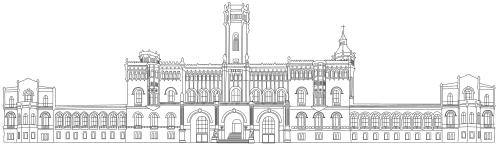
\includegraphics[height=4cm]{welfenschloss_vektor}
   \end{figure}

\vspace{1cm}

    {\LARGE \textsc{Leibniz Universität Hannover}}\\[1.0cm]

    {\Large \textsc{Institut für Antriebssysteme}} \\[0.2cm]
    {\Large \textsc{und Leistungselektronik}} \\ [0.4cm]

    {\Large \textsc{Fachgebiet Elektrische Maschinen}} \\ [0.2cm]
		{\Large \textsc{und Antriebssysteme}} \\ [1.7cm]

    {\Large \textbf{Titel \\[0.3cm] der Arbeit} } \\ [3cm]

    {\Large Diplomarbeit} \\ [1.5cm]

    {\large Vorname Name} \\
    {Matrikelnummer: xxxxxxx } \\ [1.5cm]

    \begin{tabular}{rl}
      Betreuer:    & Name Vorname\\
      Erstprüfer:  & Prof. Dr.-Ing. Bernd Ponick\\
      Zweitprüfer: & Prof. Dr.-Ing. Axel Mertens
    \end{tabular}

\end{center}

\end{titlepage}

\clearpage{\thispagestyle{empty}\cleardoublepage}       %leere Seite für "documentclass book"

\chapter*{Eigenständigkeitserklärung}
\thispagestyle{empty}
\vspace{1cm}

\begin{flushleft}

Siming Gao \\ 
Haltenhoffstraße 1 \\ 
30167 Hannover Deutschland

\vspace{1.0cm}

\begin{tabular}{@{} l l}
Matrikelnummer:  & 10026836 \\
Studienrichtung: & Elektrotechnik und Informationstechnik \\
\end{tabular}

\vspace{3.0cm}

Ich erkläre hiermit, dass ich die vorliegende Arbeit selbstständig
angefertigt und keine anderen als die angegebenen Quellen und
Hilfsmittel verwendet habe. \\ [2cm]

Hannover, den \today

\end{flushleft}


\begin{figure}[h]
	\centering
% [width=13cm]         [scale=0.9]
	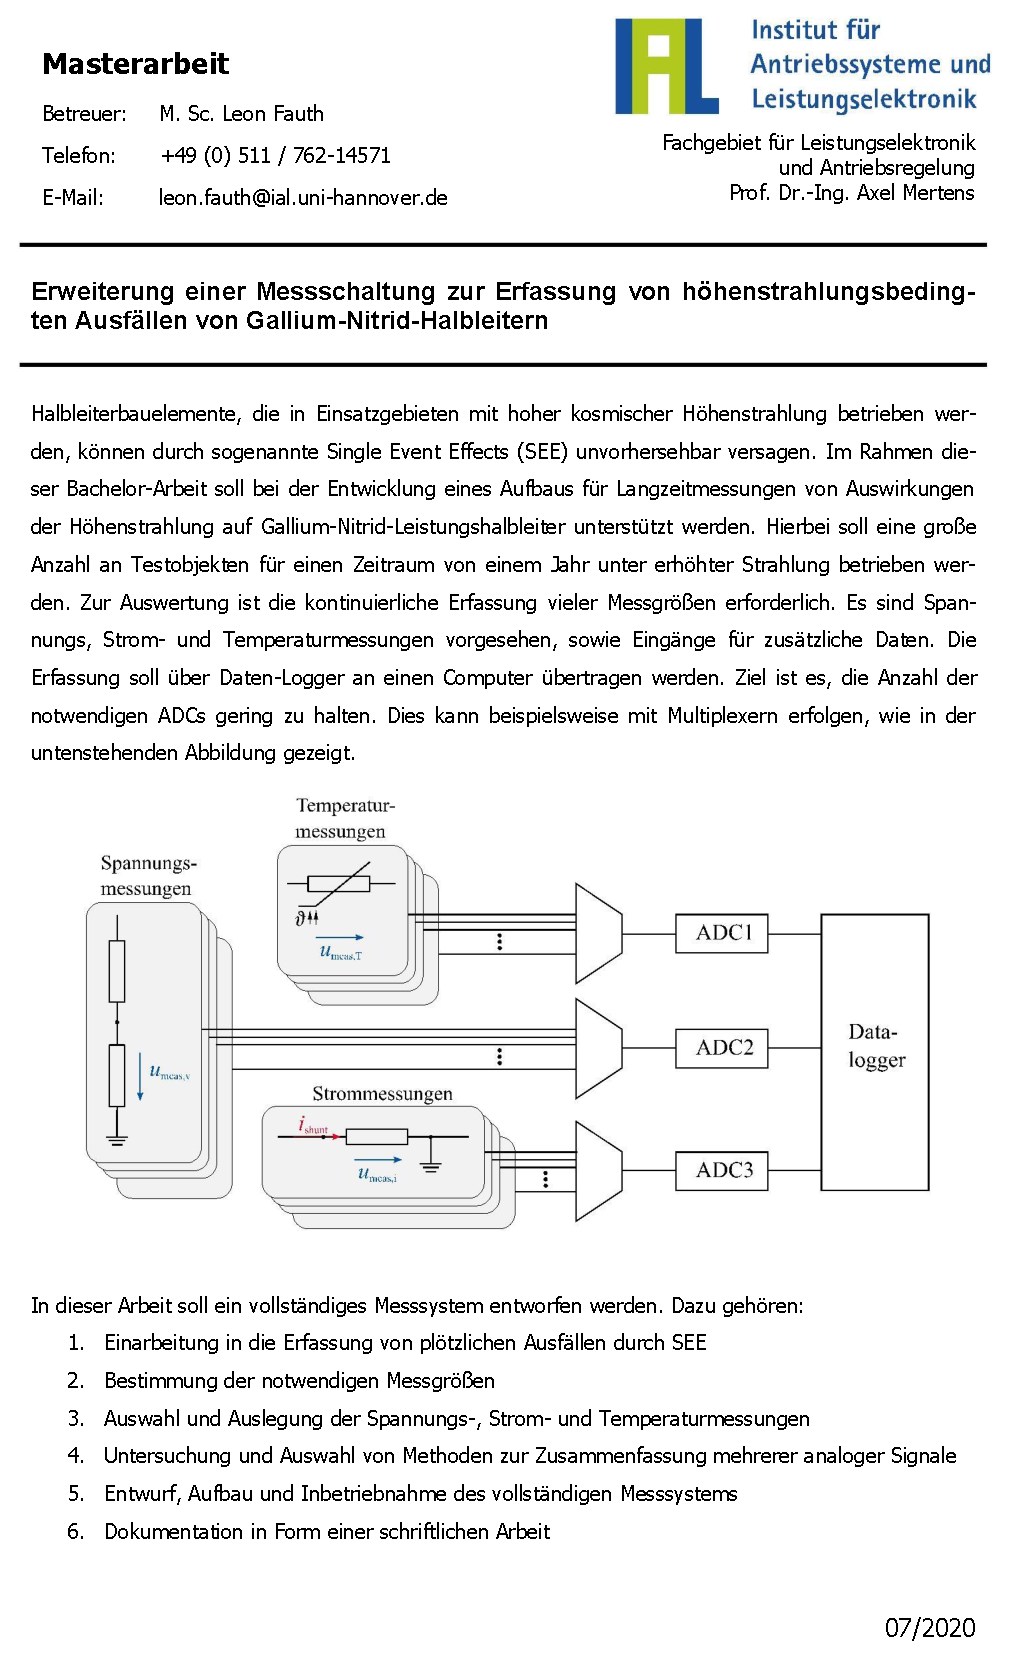
\includegraphics[scale=0.9]{grafiken/MA_Messsystem.eps}
	% \caption{Structure of divider resistor} 
	% \label{fig:2.1}
\end{figure}

\clearpage{\thispagestyle{empty}\cleardoublepage}       %leere Seite für "documentclass book"

\chapter*{Aufgabenstellung}
\thispagestyle{empty}


Hier steht die Aufgabenstellung.

\clearpage{\thispagestyle{empty}\cleardoublepage}       %leere Seite für "documentclass book"


%%%%%%%%%%%%%%%%%%%%%%%%%%%%%%%%%%%%%%%%%%%%%%%%%%%%%%%%%%%%%%%%%%%%%%%%%%%%%%%%%%%%%%%%%
%Inhaltsverzeichnis

\pagenumbering{roman}                               % Seitennummerierung arabische Zahlen
\tableofcontents
\clearpage      %leere Seite für "documentclass book"

%%%%%%%%%%%%%%%%%%%%%%%%%%%%%%%%%%%%%%%%%%%%%%%%%%%%%%%%%%%%%%%%%%%%%%%%%%%%%%%%%%%%%%%%%
%Abbildungsverzeichnis

\listoffigures
% \addcontentsline{toc}{chapter}{Abbildungsverzeichnis}   %Eintrag im InhaltsverzeichnisB
\addcontentsline{toc}{chapter}{List of figures}
\clearpage


%%%%%%%%%%%%%%%%%%%%%%%%%%%%%%%%%%%%%%%%%%%%%%%%%%%%%%%%%%%%%%%%%%%%%%%%%%%%%%%%%%%%%%%%%
%Tabellenverzeichnis

\listoftables
% \addcontentsline{toc}{chapter}{Tabellenverzeichnis}     %Eintrag im Inhaltsverzeichnis
\addcontentsline{toc}{chapter}{List of tables}   
\clearpage


%%%%%%%%%%%%%%%%%%%%%%%%%%%%%%%%%%%%%%%%%%%%%%%%%%%%%%%%%%%%%%%%%%%%%%%%%%%%%%%%%%%%%%%%%
%Formelzeichenkonvention
\markboth{Formelzeichenkonvention}{}                    %Kopfzeilenbeschriftung
\chapter*{List of Symbols}
\addcontentsline{toc}{chapter}{List of Symbols} %Eintrag im Inhaltsverzeichnis
\begin{tabular}{ll}
 
    $A$
        & Ampere\\
    $C$
        & Cycle\\
    $H$
         & Height\\
    $I$
         & Current\\
    $mAh$
        & Milliampere hour\\
    $mA$
        & Milliampere\\
    $mil$
        & Thousandth of an inch\\  
    $ms$
        & Millisecond\\
    $mV$
        & Millivolt\\
    $R$
        & Resistance\\

    $T$ & Time \\

    $U$
        & Voltage\\ 
    $V$
        & Volt\\
    $W$
        & Watt\\
    $\mu s$
        & Millisecond\\
    $\omega$
        & Ohm\\
    $\phi$ 
        &Sample command\\
\end{tabular}



%%%%%%%%%%%%%%%%%%%%%%%%%%%%%%%%%%%%%%%%%%%%%%%%%%%%%%%%%%%%%%%%%%%%%%%%%%%%%%%%%%%%%%%%%
%Formelzeichenverzeichnis

\markboth{Formelzeichenverzeichnis}{}                    %Kopfzeilenbeschriftung
%Präfix [] Konvention

%Lateinische Buchstaben bekommen im Präfix ein A
%Griechische Buchstaben bekommen im Präfix ein G
%Hochgestellte Indizes bekommen im Präfix ein X
%Indizes bekommen im Präfix ein Z
%Großbuchstaben bekommen im Präfix ein g angehängt

%Griechische Zeichen: zweistellige Nummerierung nach Stellung im Alphabet
    %alpha-01   beta-02     gamma-03    delta-04     epsilon-05   zeta-06     eta-07        theta-08
    %iota-09    kappa-10    lambda-11   mu-12        nu-13        xi-14       omicron-15    pi-16
    %rho-17     sigma-18    tau-19      upsilon-20   phi-21       chi-22      psi-23        omega-24
%Lateinische Zeichen: Lateinisches Zeichen

%\nomenclature[]{$$}{}{}{}

%%%%%%%%%%%%%%%%%%%%%%%%%%%%%%%%%%%%%%%%%%%%%%%%%%%%%%%%%%%%%%%%%%%%%%%%%%%%%%%%


\nomenclature[G03]{$\gamma$}{Kleines Gamma}{$\SI{}{\newton\meter}$}{}

\nomenclature[G03g]{$\Gamma$}{Großes Gamma}{$\SI{}{\meter\per\second}$}{}

\nomenclature[ABg]{$B$}{Großes B}{$\SI{}{\meter\per\second}$}{}

\nomenclature[Ab]{$b$}{Kleines B}{}{}

\nomenclature[ZUg]{$U$}{Großes U}{}{}

\nomenclature[Zu]{$u$}{Kleines u}{}{}

\nomenclature[XFg]{$F$}{Großes F}{}{}

\nomenclature[Xf]{$f$}{Kleines f}{}{}

\printnomenclature                                       %Verzeichnis drucken
\clearpage{\pagestyle{empty}\cleardoublepage}            %leere Seite für "documentclass book"


%%%%%%%%%%%%%%%%%%%%%%%%%%%%%%%%%%%%%%%%%%%%%%%%%%%%%%%%%%%%%%%%%%%%%%%%%%%%%%%%%%%%%%%%%
%Kapitel & Anhang

%%%%%%%%%%%%%%%%%%%%%%%%%%%%%%%%%%%%%%%%%%%%%%%%%%%%%%%%%%%%%%%%%%%%%%%%%%%%%%%%%%%%%%%%%
%Kapitel

\pagenumbering{arabic}                                  % Seitennummerierung arabische Zahlen
\chapter{Introduction}
\label{chap:Introduction}
 
\section{Importance of measurement}
\label{Importance of measurement}
% 1.1
This article is dedicated to studying the decay of gallium nitride components caused by cosmic rays and measuring the amount of gallium nitride affected by cosmic rays. And study the cause of damage to the gallium nitride transistor - whether it is related to temperature. This article measures the voltage signal and temperature signal to meet the above requirements.

\section{Motivation}
\label{Motivation}
% 1.2




\section{Introduction of measuring system}
\label{Introduction of measuring system}
% 1.3
With the advent of the digital age, digital signal processing technology has spread to all areas of daily life. In projects such as chemical engineering, medicine, industry, and scientific research, people need to detect and process the corresponding signals. People usually convert the analog signals transmitted by the sensor into digital signals according to the sampling theorem, and then process these digital signals. Data acquisition is the core of digital signal processing, and its results directly affect the follow-up work. A complete data acquisition system should include sensors, signal conditioning, data processing chips and software. The development of society and the advancement of science and technology make digital signal processing technology more and more intelligent and real-time, and the accuracy and speed of data collection are also getting higher and higher. Nowadays, many occasions such as radar measurement system, aerospace navigation, medical imaging, etc. require high-precision data acquisition, which means that people put forward higher requirements for data acquisition systems, because the measurement results in these environments need to be extremely accurate. In addition to the basic functions of data collection, people must also implement multiple functional modes, multiple range ranges, multiple control methods, etc. for different industries and different collection environments. In addition, with the rapid development of electronic technology, portable solutions have begun to occupy an increasing proportion in data acquisition, and more and more have begun to lean towards low voltage, low power consumption, and miniaturized designs. Therefore, there are more and more types of data acquisition instruments, and the update speed is getting faster and faster. General-purpose data acquisition systems cannot meet various needs in a targeted manner, which forces many companies to develop various dedicated data acquisition systems.
\\
\\
Traditional data acquisition systems mainly use data acquisition cards. In recent years, the speed of data acquisition systems and the rapid development of digital signal processing technology, while the application of USB technology, Ethernet technology and wireless communication technology in the data acquisition system has expanded its interface methods, and portable data acquisition systems have become increasingly favor of users.
The TDS-150 portable data recorder produced by Tokyo Sokki Research Institute is a static data acquisition instrument with 50 measurement channels, sleep interval timing and data storage functions, and long-term automatic measurement. It is equipped with USB and RS-233 port can read various measurement settings and measurement data and transfer them to the computer. The compact DAQ of NI Company in the United States is combined with Ethernet technology to extend the scope of high-speed data acquisition to remote sensors and electronic measurement in the laboratory and even the world. It is tightly integrated with LABVIEW software and can obtain the highest performance with less development investment.

\section{The main content of this thesis}
\label{The main content of this thesis}
% 1.4
Based on the analysis of data acquisition systems at home and abroad, this article takes into account the speed, accuracy and scalability of data acquisition, chooses the ARM M4 controller STMF429ZG and STM32F303ZET from ST Company, and designs a set of data acquisition system with strong versatility. Realize the functions of high-speed and high-precision data acquisition, display and transmission. The main research contents of this article are as follows:
\\
(1) Analyzed the research status of the data acquisition system, divided the system into different modules, studied the hardware circuit and software design of the data acquisition system based on the ARM M4 chip STM32, and initially realized the high-precision acquisition, display and transmission of signals Features.
\\
(2) Use the 12-bit precision ADC module in the Stm32 chip to collect the voltage signal and use the capture mode of the GPIO module to collect the temperature through the DS18b20 sensor, and then realize the data transmission in different single-chip computers through the SPI protocol.
\\
(3) Realize serial communication through Ethernet module.
\\
(4) Realize data display on the PC screen through IoT.
 





\chapter{Fundamentals}
\label{chap:Fundamentals}

\section{ADC}
\label{sec:ADC}
% 2.1


\subsection{How the voltage/current-sensor works}
\label{sec:How the voltage/current-sensor works}
%2.1.1

The essence of voltage/current-sensor sensor measuring voltage is a voltage divider circuit composed of resistors. Its principle is the knowledge of resistor series voltage divider. The typical circuit is shown in Figure ~\ref{fig:2.1}. 
\begin{figure}[h]
	\centering
	% \setlength\figureheight{7cm}
	% \setlength\figurewidth{13cm}
	% \input{grafiken/2.1.pdf}
	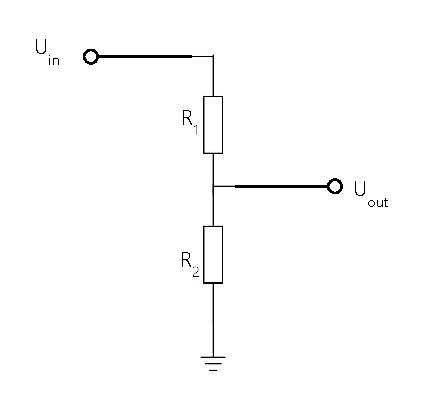
\includegraphics[width=13cm]{grafiken/2.1.pdf}
	\caption{Structure of divider resistor} 
	\label{fig:2.1}
\end{figure}
\\
$\cdot U_{in}$: Voltage of the component under test
\\
$\cdot U_{out}$: Voltage of divider resistor R2
\\
$\cdot R_{1}$: Divider resistor
\\
$\cdot R_{2}$: Divider resistor
\\
Therefore, the measured voltage provided to the ADC channel is the following formula:
\\
\begin{center} 
\begin{equation}
 U_{out} = \frac{R_{2}}{R_{1}+R_{2}} U_{in}  
\end{equation}
\end{center}

There are a variety of precision ADCs available on the market to choose from, as shown in the figure~\ref{fig:2.2} below , the appropriate ADC precision can be selected according to the signal bandwidth, so that it is convenient for users to measure.
\begin{figure}[h]
	\centering
	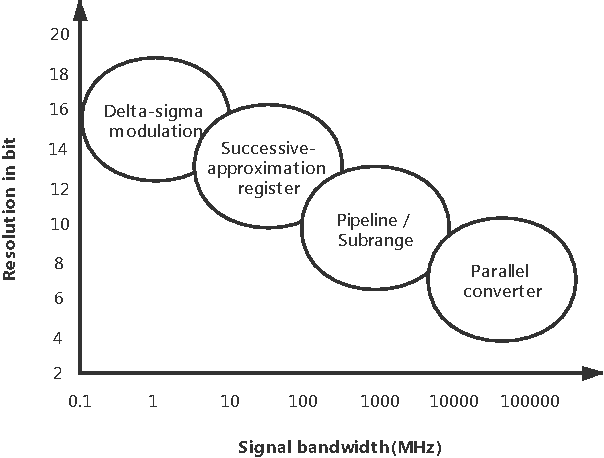
\includegraphics[width=13cm]{grafiken/2.2.pdf}
	\caption{ADC-Architecture depending on signal bandwidth and resolution} 
	\label{fig:2.2}
\end{figure}
\\
In the case of methods without feedback, the parallel converter has the simplest structure, which is why, with high resolution, a large number of components with high demands on accuracy are required. Here, too, there are methods with range selectivity, oversampling and ramp methods. A folding process has also established itself alongside a multiplex technique. 
\\
The following figure~\ref{fig:2.3} briefly describes the basic structure of the parallel converter:
\begin{figure}[h]
	\centering
	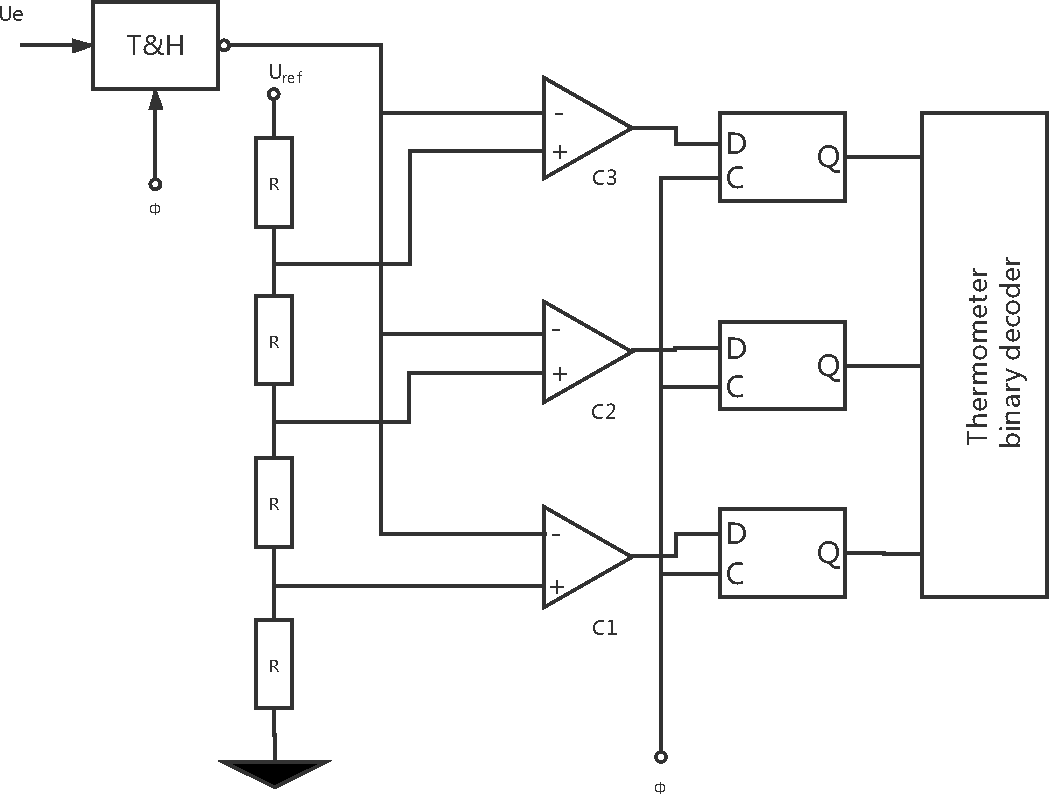
\includegraphics[width=13cm]{grafiken/2.3.pdf}
	\caption{Block diagram of a parallel converter} 
	\label{fig:2.3}
\end{figure}
\\
Since with this parallel converter (flash converter) the entire conversion takes place within one clock period, it is the fastest method. It is easy to see, however, that the number of components required quickly becomes very large, since the entire chain with resistor, comparator and latch is required for each of the $2^{n}-1$ comparison values. The thermometer code present at the output of the latches is encoded in a binary code (often a Gray code, in which neighboring numbers differ by only one bit). Differential amplifiers are particularly suitable as comparators, with the gain v having to be at least so large that $\Delta U/2$ is sufficient to control the necessary logic level of the latches.
\\
The second important method is called the weighing method, which requires feedback via a digital-to-analog converter, as Figure ~\ref{fig:2.4} shows.
\begin{figure}[h]
	\centering
	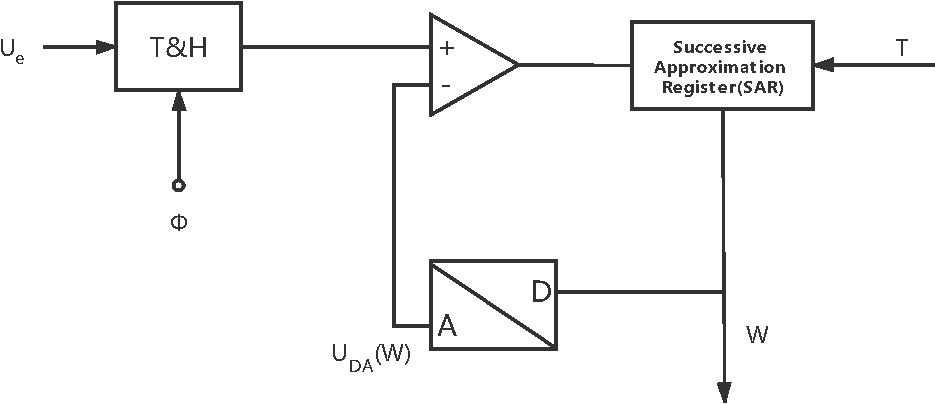
\includegraphics[width=13cm]{grafiken/2.4.pdf}
	\caption{Converter according to the weighing method} 
	\label{fig:2.4}
\end{figure}
 As soon as the track and hold element (T\&H) has switched to hold mode, the weighing cycle begins with the most significant bit. If $ u_{e}>\frac{U_{max}}{2} $, the top bit remains set and the second bit is set to 1 on a trial basis.
\\ 
The comparator decides whether the word in the SAR is smaller than the input signal. Then the check bit remains set and the next lowest bit is checked. If  $u_{e}<u_{DA}(W)$, the check bit is reset.
\\
The conversion time is n clock periods, whereby the digital-to-analog converter must have full accuracy. The advantage of high resolutions is that only one precise comparator is required. This enables the design of very energy efficient implementations.
If a counter is used instead of the SAR, the Laund can count the clock cycles backwards through the comparator. In the steady state, the data word indicates. There are also many variants of this counting method, whereby in the worst case the conversion time can be up to $2^{n}$ clock cycles.
In the gallium nitride measurement, because the precision is required but the precision is not the highest, the above-mentioned method is selected.
Each stm32F303 has a 40-channel independent 16-bit precision ADC, and the price is very high, so we choose this microcontroller to measure the voltage signal to determine whether the gallium nitride is affected by cosmic rays. The following figure~\ref{fig:2.5} is the connection diagram of the microcontroller ADC and the voltage divider resistor:
\begin{figure}[h]
	\centering
	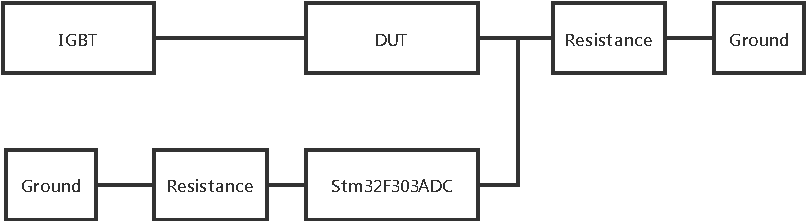
\includegraphics[width=13cm]{grafiken/2.5.pdf}
	\caption{Connection diagram of the microcontroller ADC and the voltage divider resistor} 
	\label{fig:2.5}
\end{figure}
\section{Ethernet}
\label{sec:Ethernet}
% 2.2
Ethernet has very extensive and in-depth applications in various fields and industries. This is mainly due to the high flexibility and ease of implementation of Ethernet. Because Ethernet has the advantages of simple networking, low cost, excellent compatibility, reliable connection, and convenient topology adjustment, it has advantages that other network technologies do not have in terms of being a gateway for smart homes, Internet of Things or wireless sensor networks. , Thus get vigorous development and application. This article will introduce in detail how to connect the embedded system to the Ethernet, how to use the hardware protocol stack to make your solution or application connect to the Internet quickly and efficiently, how to realize TCP/IP communication, and how to realize the upper application layer protocol and many more.
\subsection{Introduce of W5500}
\label{sec:Introduce of W5500}
% 2.2.1
The W5500 network expansion board integrates a hardware TCP/IP protocol stack chip W5500 and an RJ-45 with a network transformer. Among them, W5500 is a full hardware TCP/IP embedded Ethernet controller, which provides a simpler Internet connection solution for embedded systems. Hardware logic gate circuits are used to implement the transmission layer and network layer of the TCP/IP protocol stack (such as : TCP, UDP, ICMP, IPv4, ARP, IGMP, PPPoE and other protocols), and integrates the data link layer, physical layer, and 32K bytes of on-chip RAM as a data receiving and sending buffer. Make the host computer main control chip only need to undertake the processing task of TCP/IP application layer control information. This greatly saves the workload of the host computer for data replication, protocol processing, and interrupt processing, and improves system utilization and reliability. 
\\
Its module structure is shown in the figure~\ref{fig:2.6} below:
\\
\begin{figure}[h]
	\centering
	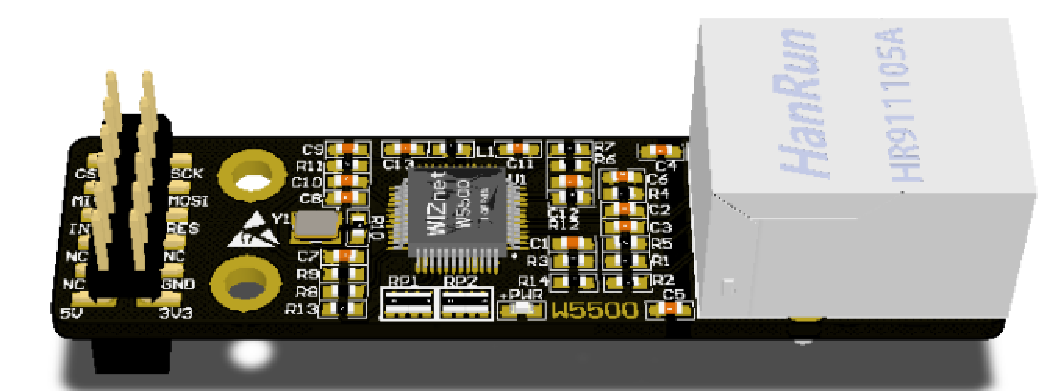
\includegraphics[width=13cm]{grafiken/2.6.pdf}
	\caption{Physical model of W5500} 
	\label{fig:2.6}
\end{figure}
W5500 supports 8 sockets at the same time to facilitate communication with different IPs and devices; in order to reduce system energy. W5500 provides Wake-on-LAN mode (WOL) and power-down mode for customers to choose to use; W5500 is non-aggressive. The hardware network engine can prevent similar torrent, fraud and injection network attacks and improve network security.

\subsection{solution of ethernet access}
\label{sec:solution of ethernet access}
% 2.2.2
For non-operating system, how does the single-chip microcomputer required by the system realize network access? I will categorize these schemes according to the different TCP/IP protocol stacks below.
\\
It is divided into two categories: the first category is the traditional software TCP/IP protocol stack solution; the second category is the latest hardware TCP/IP
Protocol stack scheme. Below I will analyze the implementation of these two types of solutions: 
\\
1) MAC+PHY solutions:

\begin{figure}[!ht]
	\centering
	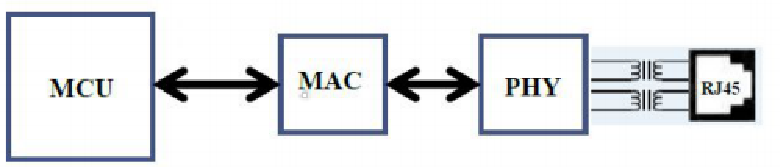
\includegraphics[width=13cm]{grafiken/2.7.pdf}
	\caption{MAC+PHY Ethernet solution} 
	\label{fig:2.7}
\end{figure}
\FloatBarrier
The traditional Ethernet access scheme is as shown in the figure below. The MCU+MAC+PHY is added to the network interface to realize the Ethernet
The physical connection of the network realizes communication and upper-layer applications by implanting TCP/IP protocol code in the main control chip.
\\
2) Hardware protocol stack chip solution: 
\begin{figure}[!ht]
	\centering
	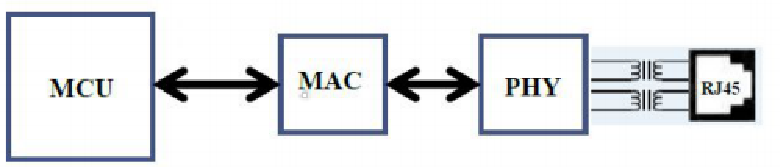
\includegraphics[width=13cm]{grafiken/2.7.pdf}
	\caption{MAC+PHY Ethernet solution} 
	\label{fig:2.8}
\end{figure}
\FloatBarrier
The hardware protocol stack chip scheme is shown in the figure below. The MCU + hardware protocol stack chip (including MAC and PHY) directly adds the network interface, and the single-chip microcomputer can be easily connected to the network. All the work of processing the TCP/IP protocol is through the "little secretary" of the MCU-the hardware protocol Stack chips to complete.
\\
This solution was first proposed by WIZnet and successfully launched the Ethernet series of chips: W5100, W5200, W5300 and W5500. The so-called hardware protocol stack refers to the implementation of the traditional software TCP/IP protocol stack with hardware-based logic gate circuits, as shown in the figure~\ref{fig:2.9} below.
\begin{figure}[!ht]
	\centering
	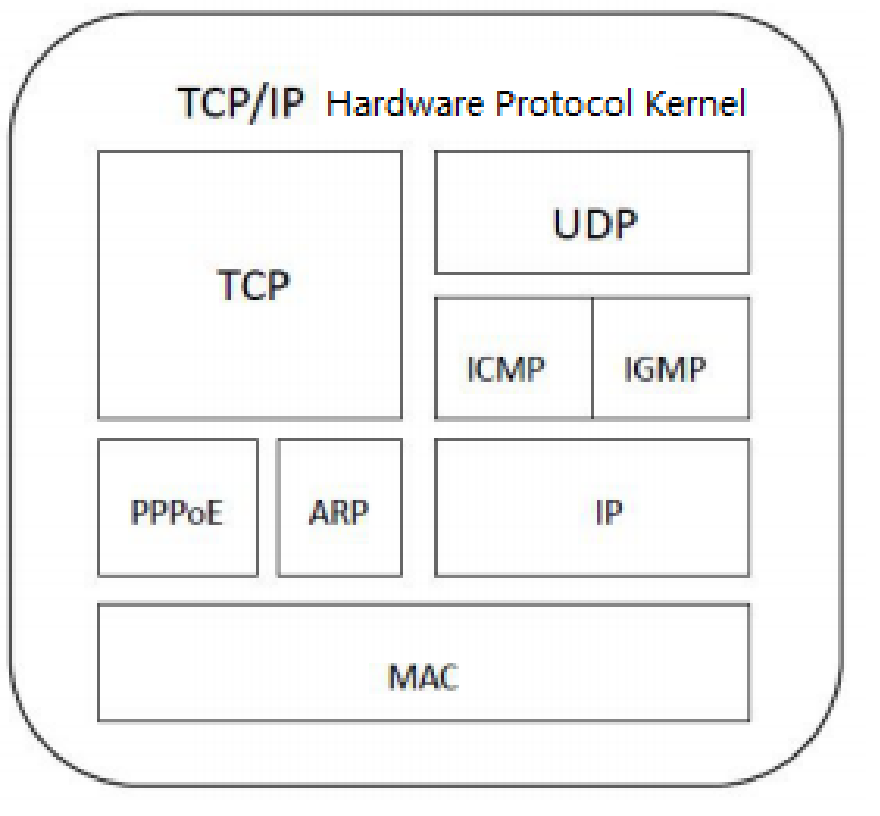
\includegraphics[width=13cm]{grafiken/2.9.pdf}
	\caption{Hardware protocol kernel} 
	\label{fig:2.9}
\end{figure}
\FloatBarrier
The core of the Ethernet chip is composed of protocols such as TCP, UDP, ICMP, IGMP in the transport layer, IP, ARP, PPPoE and other protocols in the network layer, and MAC in the link layer, plus physical layer PHY and peripheral registers and memory The SPI interface constitutes this complete set of hardware-based Ethernet solutions.
\\
This hardware TCP/IP protocol stack replaces the previous MCU to handle these interrupt requests. That is, the MCU only needs to process user-oriented application layer data. The transmission layer, network layer, link layer and physical layer are all controlled by the peripheral WIZnet The chip is complete. This set of solutions simplifies the aforementioned five-layer network model from two aspects of hardware overhead and software development, and simplifies product development solutions. In this way, engineers no longer have to face the cumbersome communication protocol code, only need to understand the simple register function and Socket programming to complete the network function development part of the product development work.

\section{Graphical user interface}
\label{sec:Graphical user interface}
% 2.3
The GUI(Graphical user interface) that separates the front and back ends specifically refers to the browser (or client) side. One of the most misunderstood concepts for novice server-side Java users is that JSP is a front-end technology. JSP needs to know the full name: Java Server Page. It runs in the servlet container on the server-side JVM, but the result of running is HTML that is responsive to the browser. Servlet, the first from Java EE, already had ASP at this point (also knows the meaning of Active Server Page). Due to the need to put a lot of HTML code in servlet, the Java specification learned ASP and suggested JSP. Servlet is Java code mixed with HTML, JSP is HTML code mixed with Java. The browser doesn't care if the server is JSP, ASP, PHP or the original servlet or HTML on the static server as long as it returns valid HTML code. So take out the static HTML part of the JSP, convert it to a simple HTML file and put it on the HTTP server. The browser just needs to fetch the HTML code. The dynamic data part is fetched by AJAX from the server side using JS in HTML and then the dom is operated dynamically to complete the display of the dynamic content. In this way, the leading and trailing ends are separated.
\\
The following figure~\ref{fig:2.10}  is the front page of the front-end:
% ~\ref{fig:2.10} 
\begin{figure}[!ht]
	\centering
	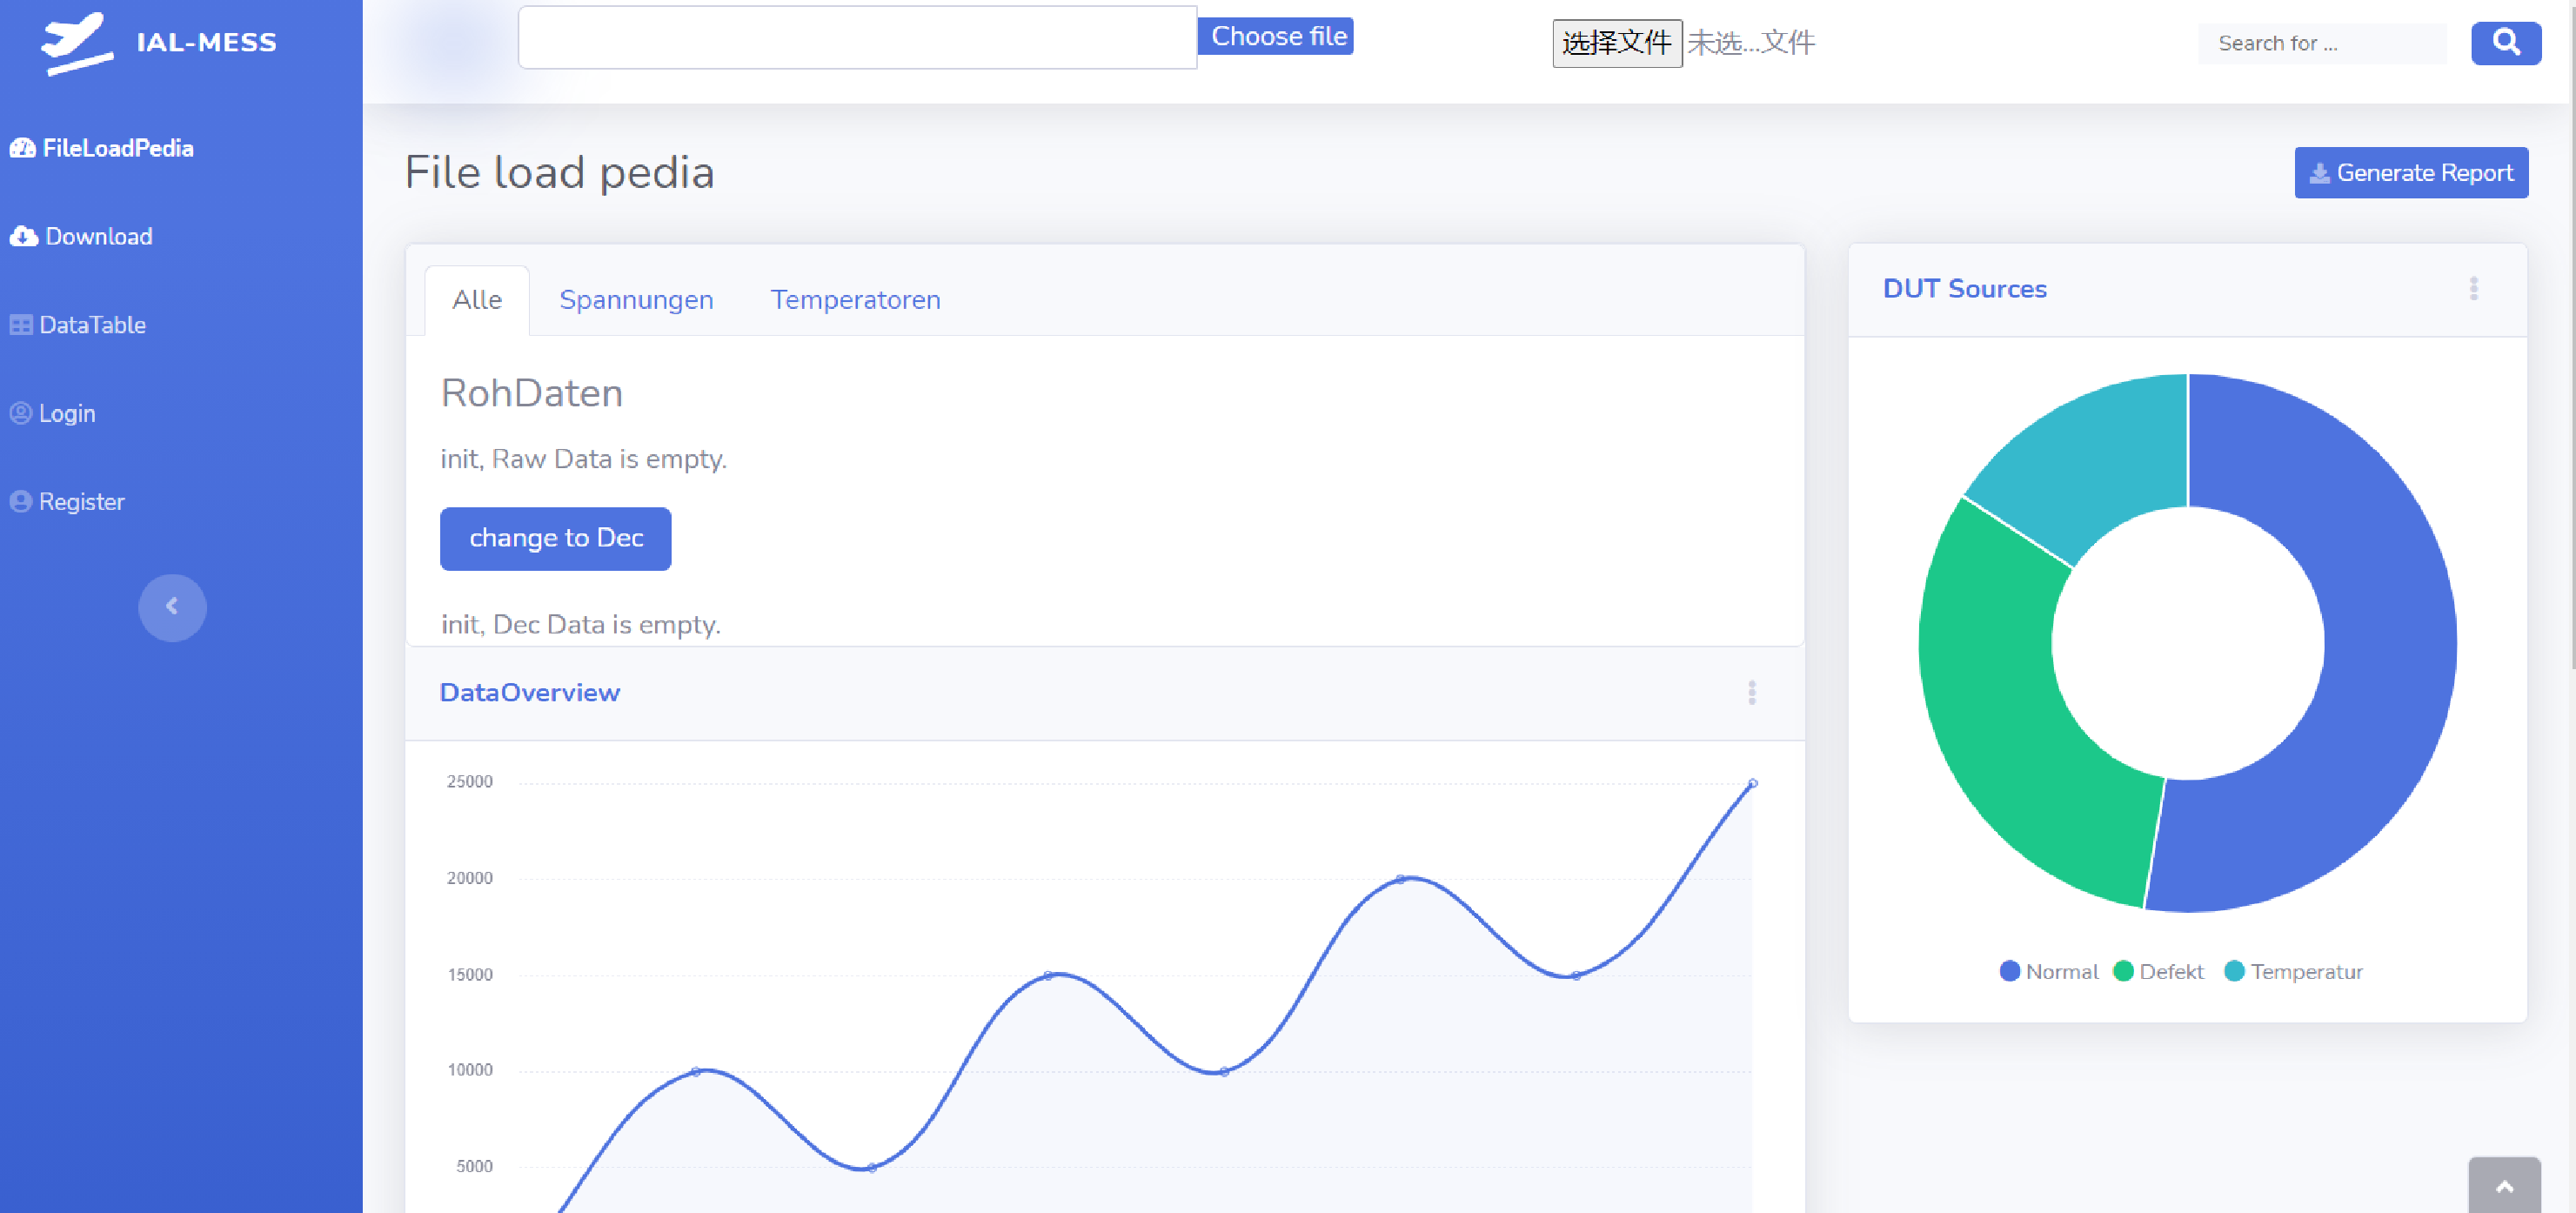
\includegraphics[width=13cm]{grafiken/2.10.pdf}
	\caption{Frontend GUI} 
	\label{fig:2.10}
\end{figure}
\FloatBarrier

\section{UDP}
\label{sec:UDP}
% 2.4
In the transport layer of the TCP/IP protocol stack, TCP is connection-oriented, and the UDP protocol to be demonstrated next. It is non-connection oriented.
\\
When UDP transmitting data, there is no confirmation, retransmission, or congestion mechanism. Since this measurement can obtain a large amount of data in a short time, the packet loss and error data can be verified by the large amount of data received later, so this time we choose UDP.
\\
Compared with TCP, UDP does not return a response signal for each received frame during transmission. When network transmission fails, such as a router restart and the network is suddenly interrupted, UDP can still receive the signal transmitted by the server as much as possible. The comparison figure~\ref{fig:2.11}  is as follows :
% ~\ref{fig:2.11} 
\begin{figure}[!ht]
	\centering
	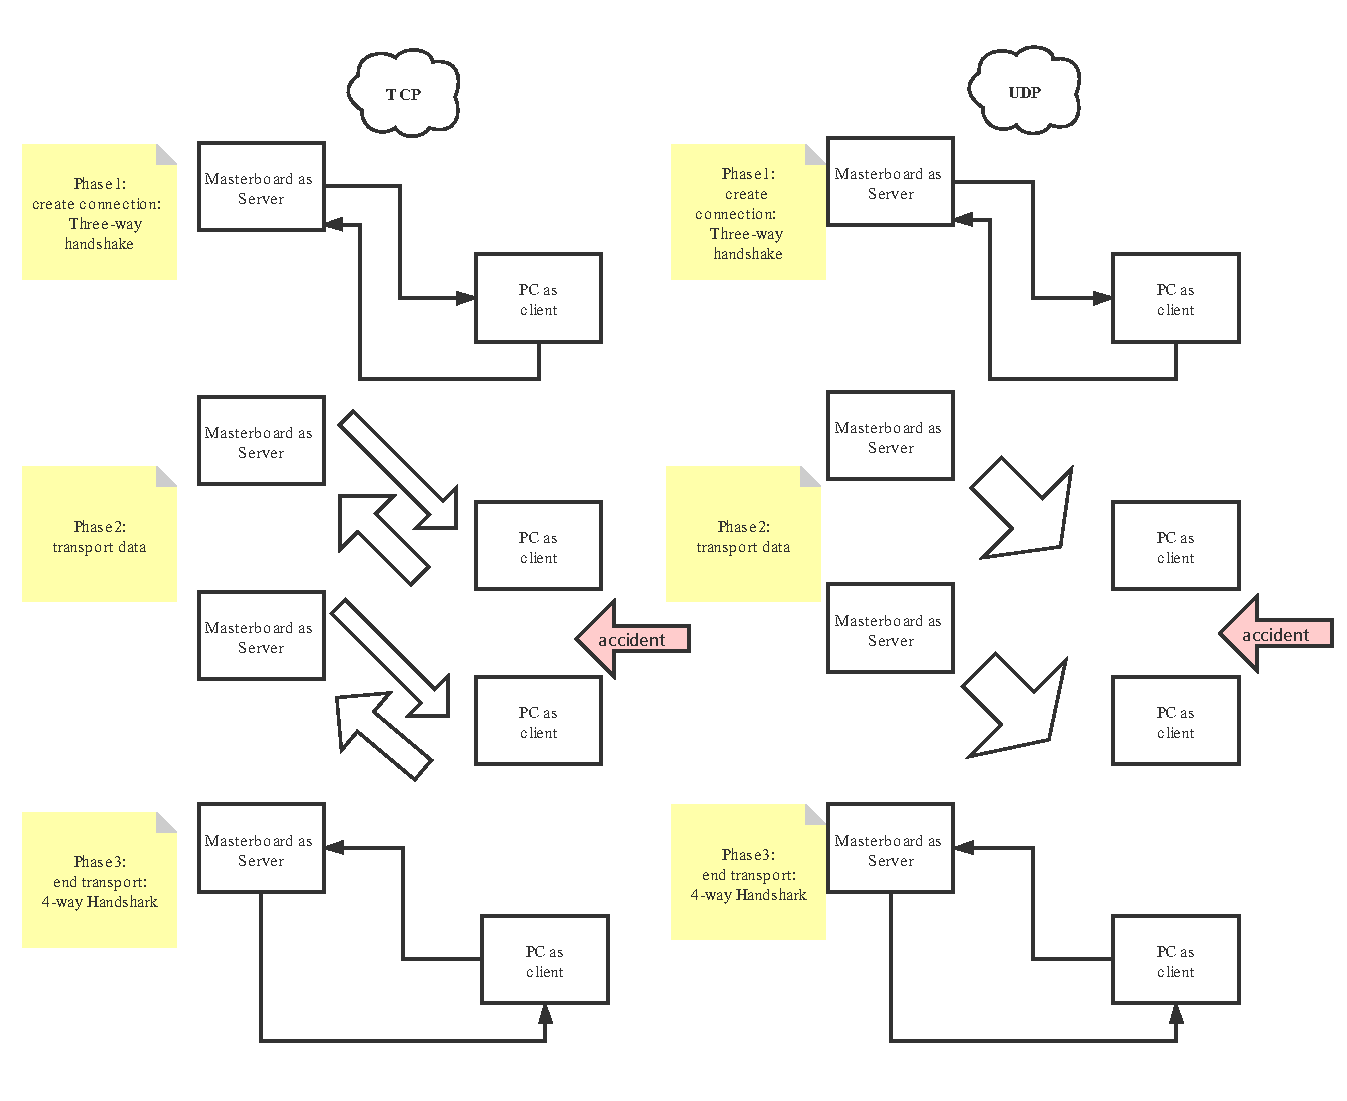
\includegraphics[width=13cm]{grafiken/2.11.pdf}
	\caption{Comparison of TCP and UDP} 
	\label{fig:2.11}
\end{figure}
\FloatBarrier
The UDP establishment process of W5500 is also very convenient, which can be easily realized by simply reading and writing registers. After the program is initialized, enter the main loop function. When the Socket is closed, before communicating, we first initialize the Socket port in UDP mode. When the socket is in the initialization completed state, that is, the SOCK UDP state, data can be sent by broadcast at this time.
\\
Next, use W5500 to demonstrate how to use UDP to send and receive data. There are two issues to pay attention to before the test. 
\\
First, it is recommended to turn off the PC firewall.
\\
Secondly, if the W5500 module and the PC are directly connected via a network cable, you need to modify the IP address of the PC to a static IP, and keep it in the same network segment as the W5500 IP. 
\\
If you connect to the router directly, you do not need to modify the IP address of the PC. The specific test steps are:
\\
1. Use the IP address obtained by the router to set the configuration file in the W5500, this IP must be in the same network segment as the router gateway.
\\
2. Obtain the computer IP address through the command line and write it as remote IP into the configuration file of the w5500 Ethernet chip.
\\
3. Compile the code, and then burn the program to the Wildfire development board.
\\
4. Connect the network cable and USB serial port cable. Open the serial port debugging tool, reset the Wildfire development board, and get the setting information from the output result.

\section{SPI}
\label{sec:SPI}
% 2.5
The Serial Peripheral Interface (SPI) is a synchronous serial communication interface specification used for short-distance communication, primarily in embedded systems. The interface was developed by Motorola in the mid-1980s and has become a de facto standard. Typical applications include Secure Digital cards and liquid crystal displays.
\\
SPI devices communicate in full duplex mode using a master-slave architecture with a single master. The master device originates the frame for reading and writing. Multiple slave-devices are supported through selection with individual slave select (SS), sometimes called chip select (CS), lines.
\\
Sometimes SPI is called a four-wire serial bus, contrasting with three-, two-, and one-wire serial buses. The SPI may be accurately described as a synchronous serial interface,[1] but it is different from the Synchronous Serial Interface (SSI) protocol, which is also a four-wire synchronous serial communication protocol. The SSI protocol employs differential signaling and provides only a single simplex communication channel. SPI is one master and multi slave communication.
\\
The figure~\ref{fig:2.12}  below is a standard SPI transmission process:
% ~\ref{fig:2.11} 
\begin{figure}[!ht]
	\centering
	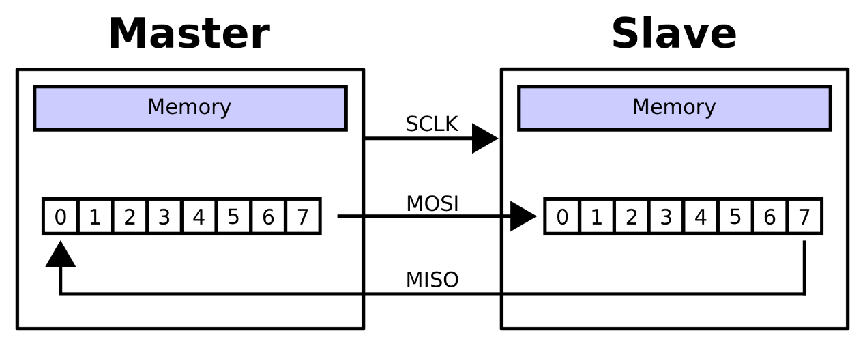
\includegraphics[width=13cm]{grafiken/2.12.pdf}
	\caption{standard SPI transmission process} 
	\label{fig:2.12}
\end{figure}
\FloatBarrier

\section{DMA}
\label{sec:DMA}
% 2.6
DMA, the full name is Direct Memory Access, that is, direct memory access.
\\
DMA transfer copies data from one address space to another address space, and provides high-speed data transfer between peripherals and memory or between memory and memory. When the CPU initializes this transfer action, the transfer action itself is realized and completed by the DMA controller. The DMA transmission method does not require the CPU to directly control the transmission, and there is no interrupt processing method to retain the scene and restore the scene process. Through the hardware, a channel for direct data transmission for RAM and IO devices is opened up, which greatly improves the efficiency of the CPU.
\\
Each channel is directly connected to a dedicated hardware DMA request, and each channel also supports software triggering. These functions are configured through software;
On the same DMA module, the priority between multiple requests can be set by software programming (a total of four levels: very high, high, medium and low). When the priority settings are equal, it is determined by the hardware (request 0 has priority over request 1, So on and so forth).
\\
The transmission width (byte, half word, full word) of the independent data source and target data area is controlled by byte in this design to simulate the process of packing and unpacking. The source and destination addresses must be aligned according to the data transfer width.
\\
DMA support circular buffer management.
\\
Each channel has 3 event flags (DMA half transfer, DMA transfer completion and DMA transfer error). These 3 event flags may logically become a separate interrupt request;
Transfer between storage and storage, between peripherals and storage, between storage and peripherals.
\\
Flash memory, SRAM, peripheral SRAM, APB1, APB2 and AHB peripherals can all be used as the source and target of access.
\\
Programmable number of data transfers: the maximum is 65535.
\\
STM32F429 series chips have up to 2 DMA controllers, DMA1 and DMA2 each have 8 channels. Each channel is dedicated to managing memory access requests from one or more peripherals. There is also an arbitration to coordinate the priority of each DMA request.
\\
Requests generated from peripherals (TIM, ADC, SPI1, SPI/I2S2, I2Cx[x=1, 2] and USART), etc., are input to the DMA1/DMA2 controller through logic OR, which means that there can only be one request at the same time effective.
The following is the working block diagram~\ref{fig:2.13}  of DMA:
% ~\ref{fig:2.12} 
\begin{figure}[!ht]
	\centering
	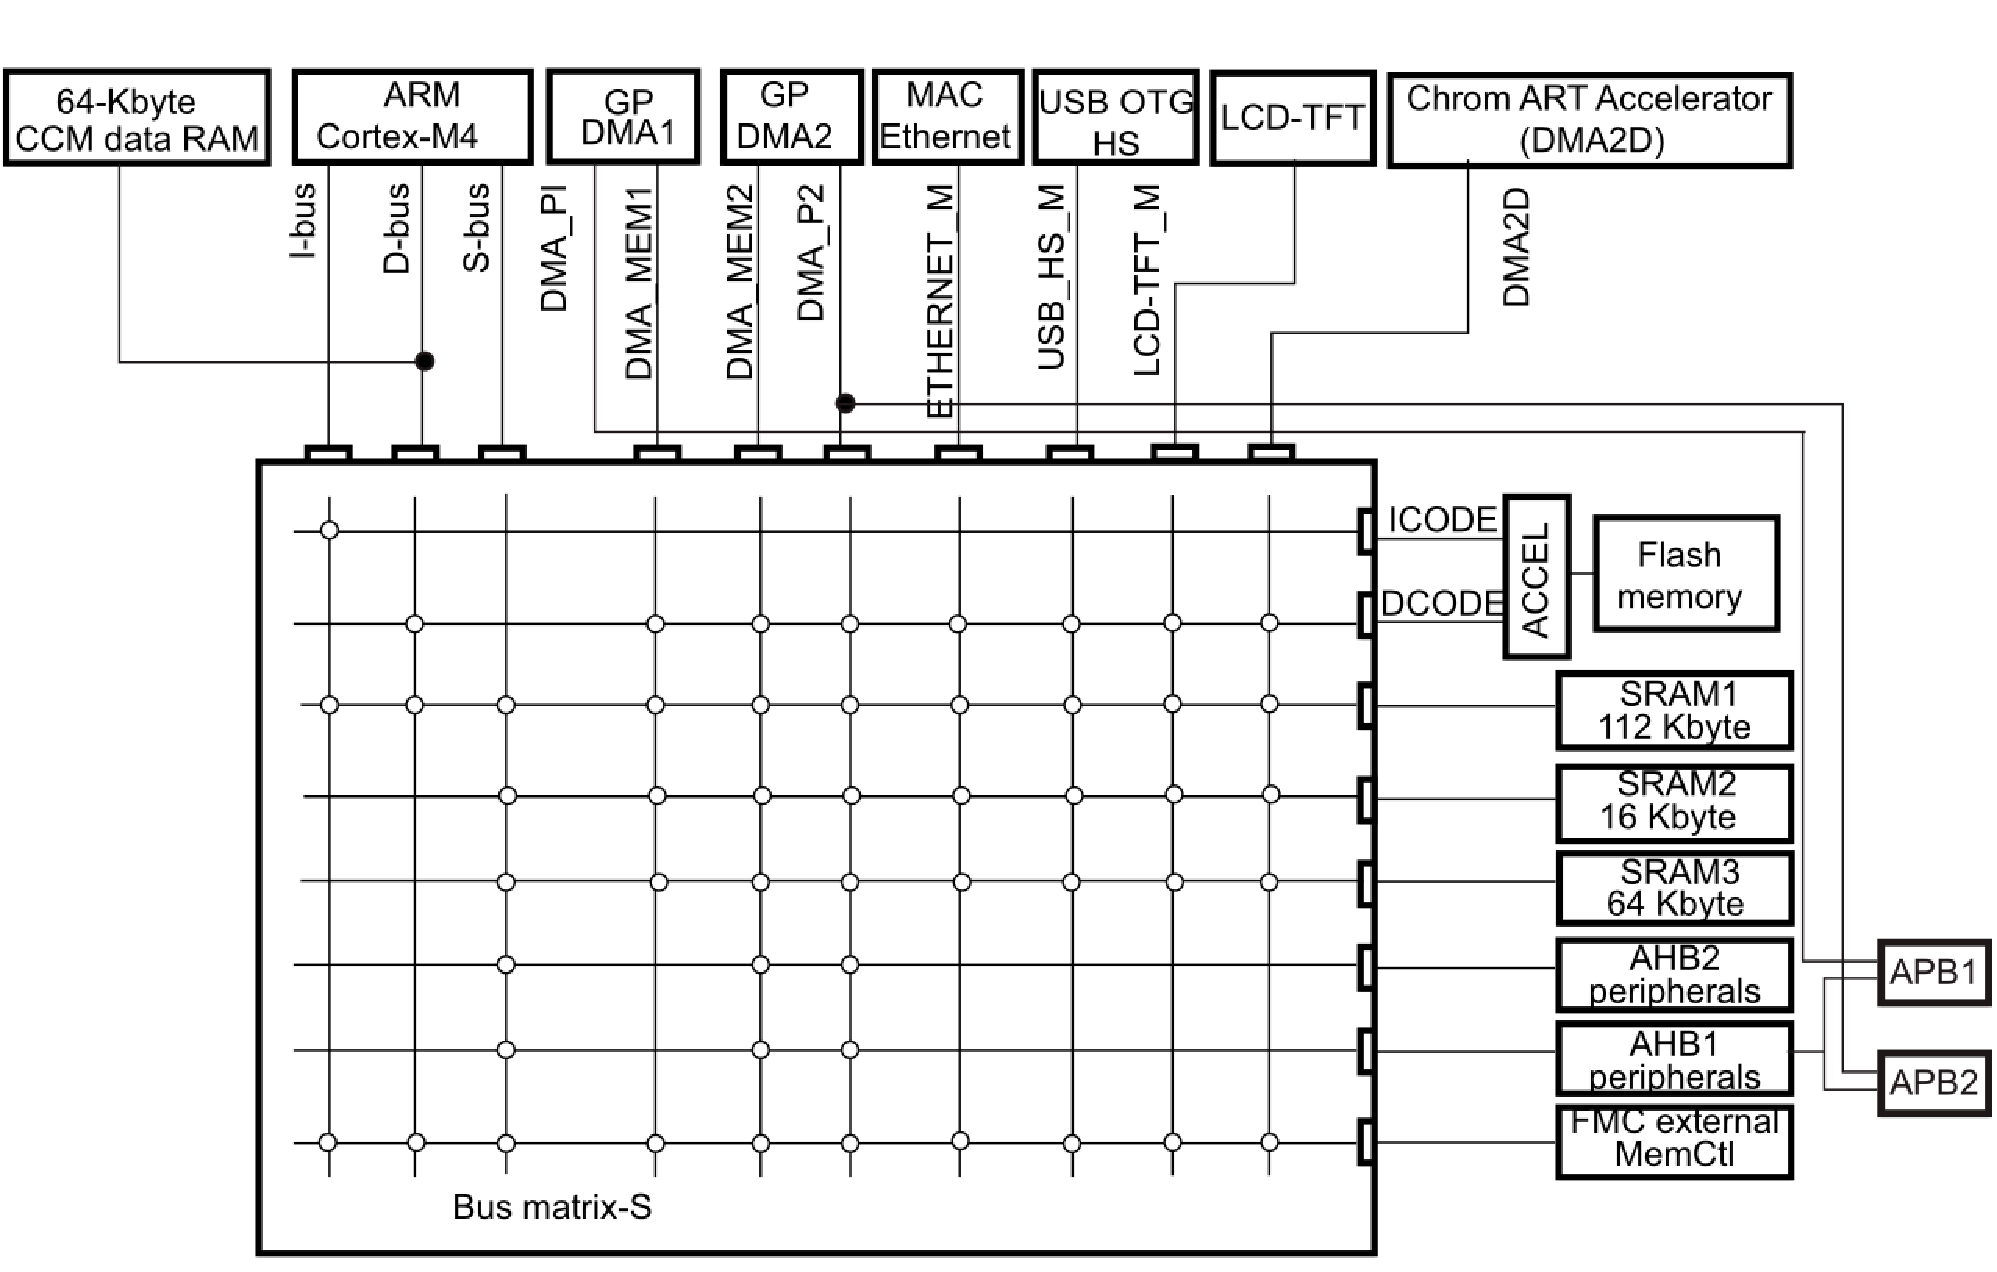
\includegraphics[width=13cm]{grafiken/2.13.pdf}
	\caption{STM32F429xx Multi-AHB matrix} 
	\label{fig:2.13}
\end{figure}
\FloatBarrier

\section{Ngrok}
\label{sec:Ngrok}
% 2.7
Intranet penetration, aka NAT penetration, is to make data packets with a specific source IP address and source port number not be shielded by the NAT device and routed to the intranet host correctly. The following describes the intranet penetration method on the relative positions of the communicating hosts on the network and the NAT device.
\\
The essence of UDP intranet penetration is to use the NAT system on the router. NAT is a conversion technology that converts private (reserved) addresses into legal IP addresses. It is widely used in various types of Internet access methods and various types of networks. NAT can complete the reuse of addresses, and can realize external concealment for the internal network structure.\\
Ngrok is a very commonly used intranet penetration technology. Usually the local PC has two IPv4 addresses, one local IP, which is assigned by the router, and one public IP. However, people in other place cannot directly access the local PC through these two IPs. If logic and data structure of the project are not complicated, developers can use the open source ngrok for intranet penetration, so that external personnel can access the local PC.\\
ngrok is a cross-platform application that enables developers to expose a local development server to the Internet with minimal effort. The software makes your locally-hosted web server appear to be hosted on a subdomain of ngrok.com, meaning that no public IP or domain name on the local machine is needed.\\
ngrok allows us to expose a web server running on your local machine to the internet. Just tell ngrok what port your web server is listening on. If you don't know what port your web server is listening on, it's probably port 80, the default for HTTP.\\
As shown in the picture~\ref{fig:2.14} , this is an example of NAT-Technical:
% ~\ref{fig:2.14} 
\begin{figure}[!ht]
	\centering
	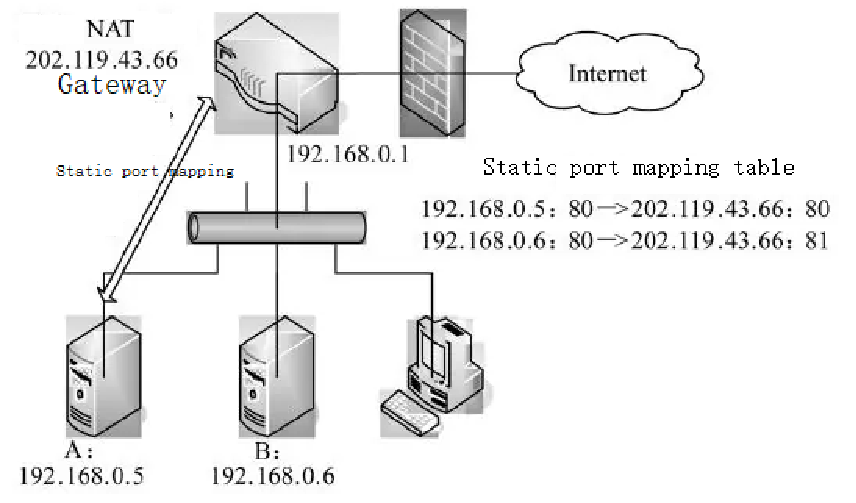
\includegraphics[width=13cm]{grafiken/2.14.pdf}
	\caption{NAT-Technical} 
	\label{fig:2.14}
\end{figure}
\FloatBarrier
This article uses Ngrok for intranet penetration, the structure is as follows~\ref{fig:2.15} :

% ~\ref{fig:2.15} 
\begin{figure}[!ht]
	\centering
	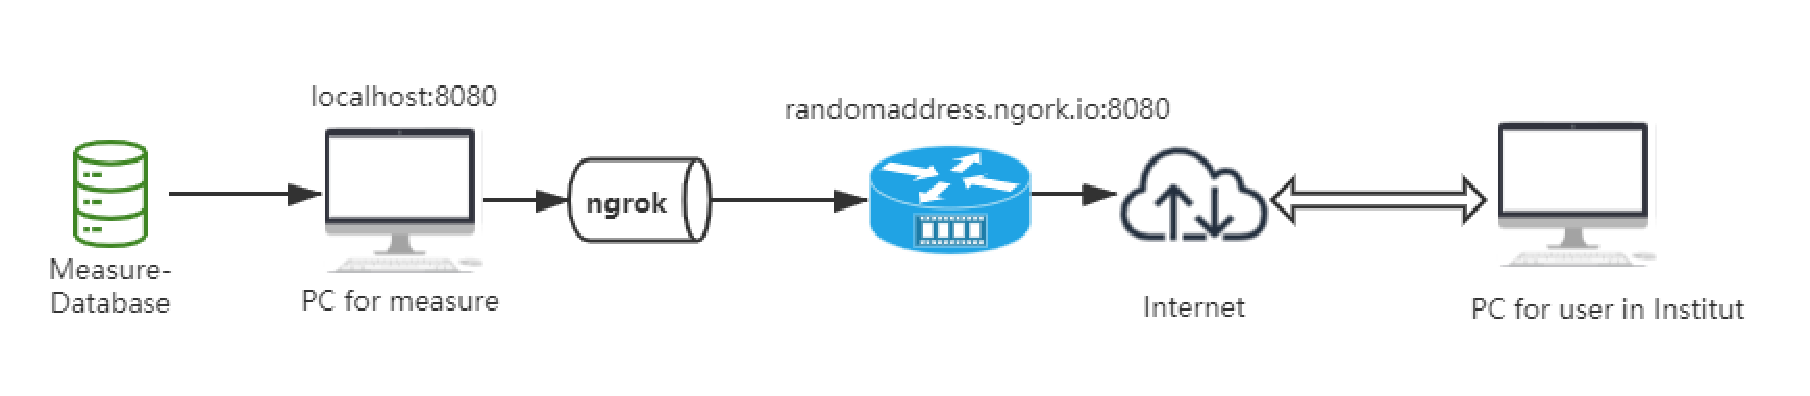
\includegraphics[width=13cm]{grafiken/2.15.pdf}
	\caption{Ngrok-Technical realization} 
	\label{fig:2.15}
\end{figure}
\FloatBarrier

\section{IoT}
\label{sec:IoT}
% 2.8
IoT is the abbreviation of English Internet of Things, it means to connect all devices to the Internet in a certain way: From smartphones and tablets (regular) to cars and refrigerators.\\
The main function of the IoT is to know how to connect devices, services, and applications to the Internet so that it can play a greater role. There are almost no restrictions, as for what devices can be connected to the IoT and the reasons for connection, \\
The important way for the IoT to improve the quality of life is to make data sharing easier: the IoT will help us to simplify our lives and can handle some trivial things for us in the long run.\\
This article uses the core concept of the Internet of Things to publish the collected data to the cloud. The user accesses the cloud server through the HTML5 page to get the pushed collected data. If the cloud server fails, the user pc can remotely control the collection PC through VNC.\\
The following figure~\ref{fig:2.16} is a schematic diagram of the Internet of Things structure used in this article:
% ~\ref{fig:2.16} 
\begin{figure}[!ht]
	\centering
	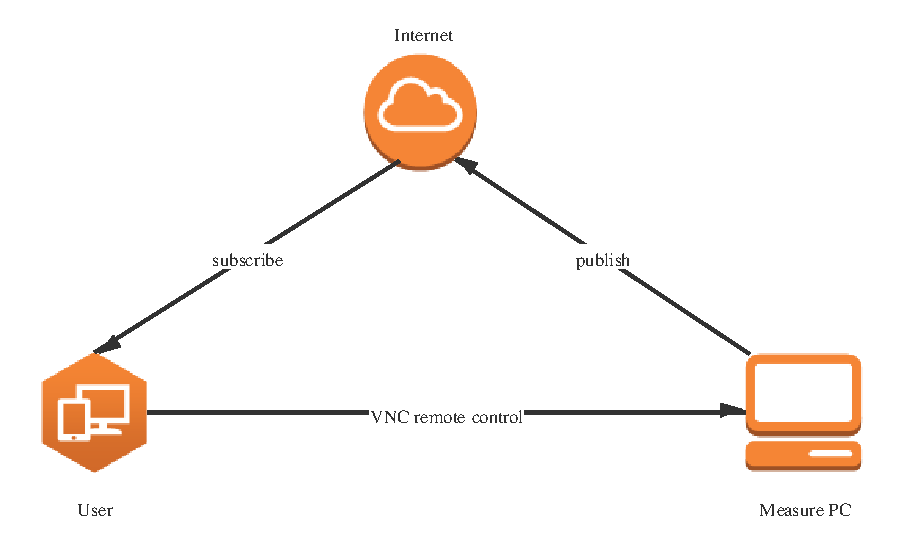
\includegraphics[width=13cm]{grafiken/2.16.pdf}
	\caption{Measuring models using the Internet of Things} 
	\label{fig:2.16}
\end{figure}
\FloatBarrier

The signal acquisition machine obtains the external network IP as a server through the intranet penetration, and collects the signal collected by the single-chip microcomputer through UDP and imports it into the database. Users or researchers in other regions can obtain it through the html web page (which has been deployed on the free website of the github page) Collect the database data of the signal machine. When there is a problem with the signal machine, the user can also remotely control the signal machine through VNC.

 
\chapter{Introduction of measurement circuit}
\label{chap:Introduction of measurement circuit}
% 3.x


\section{Measurement circuit overview}
\label{sec:Measurement circuit overview}
% 3.x
In order to ensure the measurement accuracy, we add an ADC in front of the unit under test. If the gallium nitride is affected by cosmic rays, the ADC measurement value will change from high to low to achieve the measurement purpose. The following figure shows the basic structure of the measurement system, which is blown using a fuse.

\subsection{Simulation of Measurement circuit}
\label{sec:Simulation of Measurement circuit}
% 3.x.x

\section{ }
\label{sec: }
% 3.x

\chapter{Design of the measuring system}
\label{chap:Design of the measuring system}
% 4.x

\chapter{Detailed presentation of the measuring system}
\label{chap:Detailed presentation of the measuring system}
% 5.x


\chapter{Design PCBs}
\label{chap:Design PCBs}
% 6.x

\chapter{Introduce measurement with eval boards }
\label{chap:Introduce measurement with eval boards }
% 7.x
 

\chapter{Conlusion}
\label{chap:Conlusion}
% 8.x
 

\chapter{Latex: Getting Started}
\label{chap:Latex_Getting_Started}

Zum Arbeiten mit dieser Hilfe bitte  \glqq  Arbeit.tex\grqq{} mit \textit{TexStudio} öffnen und kompilieren (F5). Anschließend kann in der PDF-Ansicht von \textit{TexStudio} per Rechtsklick auf die passende Stelle und \glqq Gehe zu Quelltext\grqq{} der zugehörige Quelltext nachgeschlagen werden. Es handelt sich hierbei nur um Minimalbeispiele um die allerersten Schritte in Latex zu schaffen.

\section{Bilder einfügen}

In Abbildung~\ref{fig:welfenschloss} ist das Welfenschloss dargestellt.
\begin{figure}[h]
	\centering
	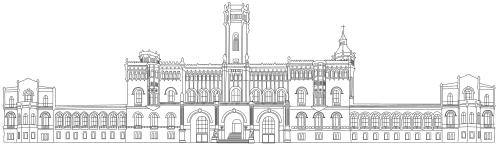
\includegraphics[width=\textwidth]{welfenschloss_vektor}
	\caption{Beispielcaption}
	\label{fig:welfenschloss}
\end{figure} 

\clearpage
\section{Plots}

\subsubsection{Gutes Beispiel}

\begin{figure}[!ht]
	\centering
	\setlength\figureheight{7cm}
	\setlength\figurewidth{13cm}
	% This file was created by matlab2tikz.
%
%The latest updates can be retrieved from
%  http://www.mathworks.com/matlabcentral/fileexchange/22022-matlab2tikz-matlab2tikz
%where you can also make suggestions and rate matlab2tikz.
%
\begin{tikzpicture}

\begin{axis}[%
width=\figurewidth,
height=0.907\figureheight,
at={(0\figurewidth,0\figureheight)},
scale only axis,
separate axis lines,
every outer x axis line/.append style={black},
every x tick label/.append style={font=\color{black}},
xmin=0,
xmax=6,
xtick={0,1,2,3,4,5,6},
xlabel={Zeit in s},
xmajorgrids,
every outer y axis line/.append style={black},
every y tick label/.append style={font=\color{black}},
ymin=-0.6,
ymax=0.6,
ytick={-0.6,-0.4,-0.2,0,0.2,0.4,0.6},
yticklabels={{-0,6},{-0,4},{-0,2},{0},{0,2},{0,4},{0,6}},
ylabel={Strom in A},
ymajorgrids,
axis background/.style={fill=white},
legend style={legend cell align=left,align=left,draw=white!15!black}
]
\addplot [color=black,solid,line width=1.0pt]
  table[row sep=crcr]{%
0	0\\
0.1	0.109268131937284\\
0.2	0.214180088269758\\
0.3	0.31055336036727\\
0.4	0.394545849994738\\
0.5	0.462809041644343\\
0.6	0.512621497281975\\
0.7	0.541997351493653\\
0.8	0.549765481672828\\
0.9	0.535616196983007\\
1	0.500113584754125\\
1.1	0.444673022100775\\
1.2	0.371504749303133\\
1.3	0.283525754501805\\
1.4	0.184243482585748\\
1.5	0.077616004432927\\
1.6	-0.0321057788851691\\
1.7	-0.140547606114757\\
1.8	-0.243386243812169\\
1.9	-0.336521840018496\\
2	-0.416241372419361\\
2.1	-0.479366674827474\\
2.2	-0.523381140639234\\
2.3	-0.546530051998406\\
2.4	-0.547890534859712\\
2.5	-0.527408351064726\\
2.6	-0.485900060646084\\
2.7	-0.425020468155793\\
2.8	-0.347196650829777\\
2.9	-0.255531198677566\\
3	-0.153678524009409\\
3.1	-0.045699171549623\\
3.2	0.0641020626677715\\
3.3	0.171347749932358\\
3.4	0.271762343126234\\
3.5	0.361342629295334\\
3.6	0.436517325117034\\
3.7	0.494289452696395\\
3.8	0.532355819617317\\
3.9	0.549198839956033\\
4	0.54414703564286\\
4.1	0.517401806173875\\
4.2	0.470029399448554\\
4.3	0.403918403830762\\
4.4	0.321704456090469\\
4.5	0.226665166882966\\
4.6	0.122589452755136\\
4.7	0.0136264839993468\\
4.8	-0.0958797296726388\\
4.9	-0.201563521088561\\
5	-0.299211610989153\\
5.1	-0.384931078176448\\
5.2	-0.45530455799711\\
5.3	-0.507526481887044\\
5.4	-0.53951492653657\\
5.5	-0.549994613602887\\
5.6	-0.538547751033225\\
5.7	-0.505630689115572\\
5.8	-0.45255572723279\\
5.9	-0.381438796627417\\
6	-0.295115104900239\\
6.1	-0.197026105230255\\
6.2	-0.0910822964965702\\
};
\addlegendentry{$i_1$};

\addplot [color=blue,dashed,line width=1.0pt]
  table[row sep=crcr]{%
0	0.242487113059643\\
0.1	0.27992203730887\\
0.2	0.248822284202539\\
0.3	0.156802157942887\\
0.4	0.0263913947523759\\
0.5	-0.110480902305586\\
0.6	-0.220303621322969\\
0.7	-0.276188330483089\\
0.8	-0.264452503936179\\
0.9	-0.187969481322183\\
1	-0.0654649740156728\\
1.1	0.0730676421006614\\
1.2	0.193710751107647\\
1.3	0.266926712344854\\
1.4	0.274789705005495\\
1.5	0.21537459425479\\
1.6	0.103228271378942\\
1.7	-0.034191932542297\\
1.8	-0.163240758891846\\
1.9	-0.252322554244172\\
2	-0.279626988260801\\
2.1	-0.238468983219033\\
2.2	-0.138925454188702\\
2.3	-0.00536812877837581\\
2.4	0.129503501776933\\
2.5	0.232668158504726\\
2.6	0.278867535444852\\
2.7	0.25679041386277\\
2.8	0.171842043088305\\
2.9	0.0448207469650515\\
3	-0.0931742311934444\\
3.1	-0.20835690799087\\
3.2	-0.272526547010924\\
3.3	-0.269972182627098\\
3.4	-0.201319212327125\\
3.5	-0.0833762775964814\\
3.6	0.0549800777391185\\
3.7	0.179875392546936\\
3.8	0.260730937885635\\
3.9	0.277750456320574\\
4	0.226766976162424\\
4.1	0.120263031464932\\
4.2	-0.0156854976550285\\
4.3	-0.147793669898183\\
4.4	-0.243716797265827\\
4.5	-0.279969552742338\\
4.6	-0.24767599742802\\
4.7	-0.154742719940931\\
4.8	-0.0239230277712742\\
4.9	0.112753855941553\\
5	0.221824663291686\\
5.1	0.276585056662421\\
5.2	0.263627781921117\\
5.3	0.1861252318252\\
5.4	0.0630527336340797\\
5.5	-0.075457272791626\\
5.6	-0.195492707173551\\
5.7	-0.267664708792873\\
5.8	-0.274303054566629\\
5.9	-0.213782445929001\\
6	-0.100920438604497\\
6.1	0.0366504118137338\\
6.2	0.165247963192162\\
};
\addlegendentry{$i_2$};

\end{axis}
\end{tikzpicture}%
	\caption{Verlauf der Str\"ome auf der Primär- und der Sekundärseite in Abh\"angigkeit von der Zeit} 
	\label{abb:stromverlauf_gutes_bsp}
\end{figure}
\FloatBarrier

\subsubsection{Schlechtes Beispiel}

\begin{figure}[!ht]
	\centering
	\setlength\figureheight{7cm}
	\setlength\figurewidth{14cm}
	% This file was created by matlab2tikz.
%
%The latest updates can be retrieved from
%  http://www.mathworks.com/matlabcentral/fileexchange/22022-matlab2tikz-matlab2tikz
%where you can also make suggestions and rate matlab2tikz.
%
\definecolor{mycolor1}{rgb}{0.00000,1.00000,1.00000}%
%
\begin{tikzpicture}

\begin{axis}[%
width=\figurewidth,
height=0.907\figureheight,
at={(0\figurewidth,0\figureheight)},
scale only axis,
separate axis lines,
every outer x axis line/.append style={black},
every x tick label/.append style={font=\color{black}},
xmin=0,
xmax=7,
xlabel={Zeit in $s$~\Huge\textcolor{red}{7}},
xmajorgrids,
every outer y axis line/.append style={black},
every y tick label/.append style={font=\color{black}},
ymin=-0.5,
ymax=0.5,
ytick={-0.4, -0.2,    0,  0.2,  0.4},
ylabel={Strom [A]~\Huge\textcolor{red}{1}},
ymajorgrids,
axis background/.style={fill=white},
legend style={at={(0.03,0.97)},anchor=north west,legend cell align=left,align=left,draw=white!15!black}
]
\addplot [color=blue,solid,line width=1.0pt]
  table[row sep=crcr]{%
0	0\\
0.1	0.0894011988577775\\
0.2	0.175238254038893\\
0.3	0.254089113027766\\
0.4	0.322810240904785\\
0.5	0.378661943163553\\
0.6	0.419417588685252\\
0.7	0.443452378494807\\
0.8	0.449808121368677\\
0.9	0.438231433895188\\
1	0.409183842071557\\
1.1	0.363823381718816\\
1.2	0.303958431248018\\
1.3	0.231975617319659\\
1.4	0.150744667570157\\
1.5	0.0635040036269403\\
1.6	-0.026268364542411\\
1.7	-0.114993495912074\\
1.8	-0.199134199482684\\
1.9	-0.275336050924224\\
2	-0.340561122888568\\
2.1	-0.392209097586115\\
2.2	-0.428220933250282\\
2.3	-0.447160951635059\\
2.4	-0.448274073976128\\
2.5	-0.431515923598412\\
2.6	-0.397554595074069\\
2.7	-0.347744019400194\\
2.8	-0.284069987042544\\
2.9	-0.20907098073619\\
3	-0.125736974189517\\
3.1	-0.0373902312678734\\
3.2	0.0524471421827221\\
3.3	0.14019361358102\\
3.4	0.222351008012374\\
3.5	0.295643969423455\\
3.6	0.357150538732119\\
3.7	0.404418643115232\\
3.8	0.435563852414169\\
3.9	0.449344505418572\\
4	0.445211210980522\\
4.1	0.423328750505898\\
4.2	0.384569508639726\\
4.3	0.330478694043351\\
4.4	0.263212736801293\\
4.5	0.18545331835879\\
4.6	0.100300461345111\\
4.7	0.011148941454011\\
4.8	-0.0784470515503408\\
4.9	-0.164915608163368\\
5	-0.244809499900216\\
5.1	-0.314943609417094\\
5.2	-0.372521911088544\\
5.3	-0.415248939725763\\
5.4	-0.441421303529921\\
5.5	-0.449995592947817\\
5.6	-0.440629978118093\\
5.7	-0.413697836549104\\
5.8	-0.370272867735919\\
5.9	-0.312086288149705\\
6	-0.241457813100196\\
6.1	-0.161203177006572\\
6.2	-0.0745218789517392\\
};
\addlegendentry{i$_1$};

\addplot [color=mycolor1,solid,line width=1.0pt]
  table[row sep=crcr]{%
0	0.242487113059643\\
0.1	0.27992203730887\\
0.2	0.248822284202539\\
0.3	0.156802157942887\\
0.4	0.0263913947523759\\
0.5	-0.110480902305586\\
0.6	-0.220303621322969\\
0.7	-0.276188330483089\\
0.8	-0.264452503936179\\
0.9	-0.187969481322183\\
1	-0.0654649740156728\\
1.1	0.0730676421006614\\
1.2	0.193710751107647\\
1.3	0.266926712344854\\
1.4	0.274789705005495\\
1.5	0.21537459425479\\
1.6	0.103228271378942\\
1.7	-0.034191932542297\\
1.8	-0.163240758891846\\
1.9	-0.252322554244172\\
2	-0.279626988260801\\
2.1	-0.238468983219033\\
2.2	-0.138925454188702\\
2.3	-0.00536812877837581\\
2.4	0.129503501776933\\
2.5	0.232668158504726\\
2.6	0.278867535444852\\
2.7	0.25679041386277\\
2.8	0.171842043088305\\
2.9	0.0448207469650515\\
3	-0.0931742311934444\\
3.1	-0.20835690799087\\
3.2	-0.272526547010924\\
3.3	-0.269972182627098\\
3.4	-0.201319212327125\\
3.5	-0.0833762775964814\\
3.6	0.0549800777391185\\
3.7	0.179875392546936\\
3.8	0.260730937885635\\
3.9	0.277750456320574\\
4	0.226766976162424\\
4.1	0.120263031464932\\
4.2	-0.0156854976550285\\
4.3	-0.147793669898183\\
4.4	-0.243716797265827\\
4.5	-0.279969552742338\\
4.6	-0.24767599742802\\
4.7	-0.154742719940931\\
4.8	-0.0239230277712742\\
4.9	0.112753855941553\\
5	0.221824663291686\\
5.1	0.276585056662421\\
5.2	0.263627781921117\\
5.3	0.1861252318252\\
5.4	0.0630527336340797\\
5.5	-0.075457272791626\\
5.6	-0.195492707173551\\
5.7	-0.267664708792873\\
5.8	-0.274303054566629\\
5.9	-0.213782445929001\\
6	-0.100920438604497\\
6.1	0.0366504118137338\\
6.2	0.165247963192162\\
};
\addlegendentry{$i_2$};
\node[font=\bfseries] at (0.2,-0.42) {\Huge\textcolor{red}{2}};
\node[font=\bfseries] at (1,0.45) {\Huge\textcolor{red}{3}};
\node[font=\bfseries] at (1,0.34) {\Huge\textcolor{red}{4}};
\node[font=\bfseries] at (6.5,0.4) {\Huge\textcolor{red}{5}};
\node[font=\bfseries] at (6.5,0) {\Huge\textcolor{red}{6}};
\node[font=\bfseries] at (2.2,0.07) {\Huge\textcolor{red}{9}};
\end{axis}
\end{tikzpicture}%
	\caption{Str\"ome in Abh\"angigkeit der Zeit~\Huge\textcolor{red}{8}} 
	\label{abb:stromverlauf_schlechtes_bsp}
\end{figure}
\FloatBarrier
\newpage


\subsubsection{Erläuterungen zum Plot}

\begin{enumerate}
	\item[1)] Einheiten nicht in eckige Klammer schreiben. Richtig ist:
	\begin{itemize}
		\item Strom in A
		\item Strom /A
		\item Strom $i$ in A
		\item Strom $i$ /A
		\item $i$ in A
		\item $i$ /A
		\item Wichtig ist: immer eine einheitliche Darstellung verwenden
		\item zur Info: diese Schreibweise ist korrekt: [$i$]~=~A, wird aber nicht als Achsenbeschriftung verwendet
	\end{itemize}
	\item[2)] In deutschen Arbeiten Dezimalkomma verwenden. In englischen Veröffentlichungen Dezimalpunkte verwenden.
	\item[3)] Indizes gerade (es sei denn, der Index ist eine Variable, z.B. Zählvariable)
	\item[4)] Legende muss an einer günstigen Stelle platziert sein, möglichst Verdeckung vermeiden
	\item[5)] Abbildung darf nicht über den Rand des Dokuments ragen
	\item[6)] Verläufe sollten bis zum Ende des Plots gehen. Die Achse muss nicht zwingend mit einem Zahlenwert abgeschlossen werden.
	\item[7)] Einheiten immer gerade schreiben, nicht kursiv
	\item[8)] Es heißt immer: in Abhängigkeit \textbf{von} ...
	\item[9)] Geeignete Plotfarben wählen, die gut erkennbar sind. Für s/w-Ausdrucke ist es sinnvoll auch die Art des Plots zu unterscheiden (durchgezogen, gestrichelt, gepunktet, markiert)
\end{enumerate}

\subsubsection{Tipps}

\begin{itemize}
	\item Bildunterschrift muss vollständig und eindeutig sein
	\item Möglichst nicht mehr als drei bis vier Verläufe pro Plot abbilden
	\item Skalierung der Achsen sinnvoll wählen
\end{itemize}

\section{Tabellen}

Tabellen sind recht umfangreich und etwas aufwendiger als in Word. Gute Beispiele gibt es unter anderem hier: \href{https://en.wikibooks.org/wiki/LaTeX/Tables}{https://en.wikibooks.org/wiki/LaTeX/Tables}.

\section{Gleichungen}

\subsection{Einheiten}
Einheiten sind nicht kursiv zu schreiben. Da dies innerhalb der Mathematikumgebung häufig schief geht, wird empfohlen den Befehl \verb=$\SI{40}{\N\m}$= zu verwenden. Die Darstellung von Einheiten kann dadurch global eingestellt werden (immer gerade, Einheiten mit Bruchstrich oder negativen Exponenten, Komma als Dezimaltrenner, usw.).

Beispiel:

Damit beträgt das Drehmoment beträgt $M=\SI{40}{\N\m}$.

Weitere Beispiele:
\begin{enumerate}
	\item $\SI{1}{\meter\per\square\second}$
	\item $\SI{100}{\nano\farad}$
	\item $\SI{100}{\mega\var}$
\end{enumerate}
Neue Einheiten können über  \verb!\DeclareSIUnit \var {var}! in \glqq  Pakete.tex\grqq{} erstellt werden.

\section{Literaturverweise setzen}

In \cite{ASYN:2001} sind die notwendigen Formeln dargestellt.
% \documentclass[11pt, oneside]{article}   	% use "amsart" instead of "article" for AMSLaTeX format
% \usepackage{geometry}                		% See geometry.pdf to learn the layout options. There are lots.
% \geometry{letterpaper}                   		% ... or a4paper or a5paper or ... 
% %\geometry{landscape}                		% Activate for rotated page geometry
% %\usepackage[parfill]{parskip}    		% Activate to begin paragraphs with an empty line rather than an indent
% \usepackage{graphicx}				% Use pdf, png, jpg, or eps§ with pdflatex; use eps in DVI mode
% 								% TeX will automatically convert eps --> pdf in pdflatex		
% \usepackage{amssymb}

%SetFonts

%SetFonts


% \title{Brief Article}
% \author{The Author}
% %\date{}							% Activate to display a given date or no date

% \begin{document}
% \maketitle
% %\section{}
% %\subsection{}



% \end{document} 
\chapter{Auswertung}
\label{chap:Auswertung}


% Im folgenden Kapitel


%%%%%%%%%%%%%%%%%%%%%%%%%%%%%%%%%%%%%%%%%%%%%%%%%%%%%%%%%%%%%%%%%%%%%%%%%%%%%%%%%%%%%%%%%
%Anhang
\clearpage{\thispagestyle{empty}\cleardoublepage}				% Anhang auf rechter Seite beginnen
\begin{appendix}
\chapter{Motordaten}
\label{app:Motordaten}

Im Folgenden  111111
\end{appendix}


%%%%%%%%%%%%%%%%%%%%%%%%%%%%%%%%%%%%%%%%%%%%%%%%%%%%%%%%%%%%%%%%%%%%%%%%%%%%%%%%%%%%%%%%%
%Literaturverzeichnis

\bibliography{Literaturverzeichnis}
\clearpage

%%%%%%%%%%%%%%%%%%%%%%%%%%%%%%%%%%%%%%%%%%%%%%%%%%%%%%%%%%%%%%%%%%%%%%%%%%%%%%%%%%%%%%%%%
%Ende des Dokuments
\end{document} 